\documentclass{article}
\usepackage[T2A]{fontenc}
\usepackage[utf8]{inputenc}
\usepackage[russian]{babel}
\usepackage{amscd}
\usepackage[inline]{enumitem}
\usepackage{amsmath}
\usepackage{dsfont}
\usepackage{indentfirst}
\usepackage{amssymb}
\usepackage{amsfonts}
\usepackage{amsthm}
\usepackage{epigraph}
\usepackage{icomma}
\renewcommand{\thesection}{\arabic{section}}
\renewcommand{\baselinestretch}{1.0}
\renewcommand\normalsize{\sloppypar}
\setlength{\topmargin}{-0.5in} 
\setlength{\textheight}{9.1in}
\setlength{\oddsidemargin}{-0.3in}
\setlength{\textwidth}{7in}
\setlength{\parindent}{0ex}
\setlength{\parskip}{1ex}
%Image-related packages
\usepackage[dvipsnames]{xcolor}
\usepackage[table]{xcolor}
\usepackage{graphicx}
\usepackage{caption}
\usepackage{subcaption}
\usepackage[export]{adjustbox}
\usepackage{wrapfig}
\title{Прикладная теория графов\\Зачетные задачи}
\author{4 курс 61 группа\\Доний Кира}
\date{VII семестр, 2024}
\graphicspath{{attachments/}}
\begin{document}
\maketitle

\clearpage% 1------------------------------------------
\begin{enumerate} 
\item[\textbf{Задача 1.}] Построить орграф, который включает не менее 10 вершин и 20 дуг, являющийся моделью, некоторой прикладной задачи. Провести анализ данного графа (определить сильные компоненты, базы, антибазы; построить иерархию) и интерпретировать полученные результаты.
\\
\textit{Прикладная задача:}\\
На графе, представленном на рисунке \ref{fig:1_graph}, отражена организация управления некоторой фирмы. Проанализировать граф и интерпретировать полученные результаты.
\begin{figure}[h]
    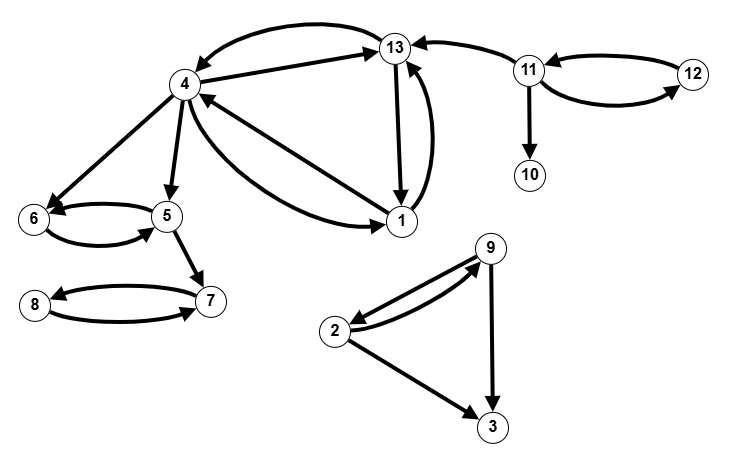
\includegraphics[width=0.7\textwidth, center]{attachments/1/0.png}
    \caption{Граф производственных отношений}
    \label{fig:1_graph}
\end{figure}
\begin{center}
Решение 
\end{center}

\begin{itemize}
    \item Сильные компоненты.\\
    Для определения сильных компонент используем алгоритм, представленный ниже.
    Подробно по шагам процесс представлен на рисунке \ref{fig:1_sk}.
    \begin{enumerate}
        \item[\textbf{S1}] Орграф $G = (X,U)$. Выберем произвольную вершину $x_0$, построим множества достижимости $R(x_0) = \{x_i : x_0 \rightarrow\rightarrow x_i\}$ и контрдостижимости $Q(x_0) = \{x_i : x_i \rightarrow\rightarrow x_0\}$.  \\
        \item[\textbf{S2}] Определим сильную компоненту, содержащую $x_0$ как $\text{СК}(x_0) = R(x_0) \cap Q(x_0)$\\.
        \item[\textbf{S3}] Удалить из графа вершины, входящие в $\text{СК}(x_0)$.\\
        \item[\textbf{S4}] Повторить шаги S1-S2, пока граф не пуст.\\
    \end{enumerate}
  
    \item База и антибаза.\\
    Для нахождения базы и антибазы найдем для начала конденсацию графа. С учетом представленного выше разложения на сильные компоненты конденсация имеет вид, представленный на рисунке \ref{fig:1_condenc}. \\
    В базу конденсации входят те вершины, которые не имеют входящих дуг, то есть $B^* = \{CK_5,CK_4\}$. Соответственно, база графа:
    $B = \{\{2,11\},\{2,12\},\{9,11\},\{9,12\}\}$ \\
    В антибазу конденсации входят те вершины, которые не имеют входящих дуг, то есть $\overline{B}^* = \{CK_3,CK_6,CK_7\}$. Соответственно, антибаза графа: $\overline{B} = \{\{7,10,3\},
    \{8,10,3\}\}$
\begin{figure}[h]
    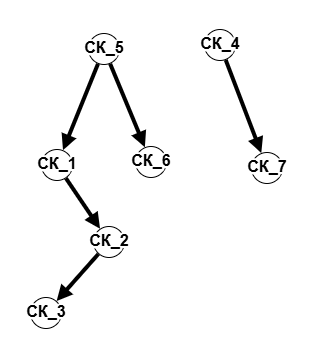
\includegraphics[width=0.3\textwidth, center]{attachments/1/condens_1.png}
    \caption{Конденсация}
    \label{fig:1_condenc}
\end{figure}
    \item Иерархия.\\
    Для выявления иерархии воспользуемся конденсацией, построенный в пункте выше.
    \item Интерпретация.\\
    Интерпретируем полученные результаты: \textit{сильные компоненты} показывают, что две вершины имеют влияние друг на друга, что может свидетельствовать о работе на одном уровне организации людей, отмеченных вершинами, входящих в одну сильную компоненту. Предполагаемый вариант - коллеги одной специальности.
    \textit{База} графа показывает людей, обладающих высшей организационной властью, \textit{антибаза} - наоборот. Можем предположить, что вершинам антибазы соответствуют стажеры, а базы - менеджеры высшего звена.
    \textit{Иерархия} в примере организации интерпретируема как иерархия власти.

    
\begin{table}[ht]
    \centering
    \begin{tabular}{c|c}
    \hline
    \textit{Уровень} & \textit{Сильные компоненты} \\ \hline
    1 & СК5, СК4 \\
    2 & СК1, СК6, СК7 \\
    3 & СК2 \\
    4 & СК3 \\ \hline
    \end{tabular}
    \caption{Иерархия}
    \label{tab:1_ierarchy}
\end{table}

\end{itemize}

\begin{figure}[ht]
     \centering
     \begin{subfigure}[t]{0.47\textwidth}
        \centering
         \caption*{\small{$x_0 := 1$\quad
            $R(1)=\{1,4,5,6,7,8,13\}$\\$Q(1)=\{1,4,11,12,13\}$\qquad\qquad
            $\text{СК}(1) = \{1,4,13\}$}}
         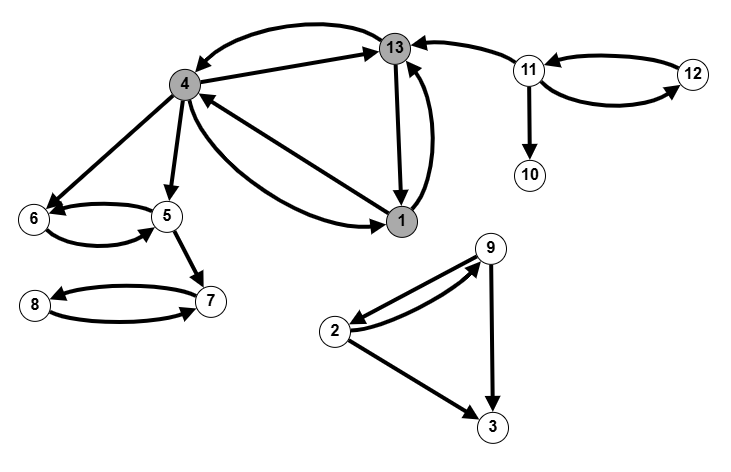
\includegraphics[width=\textwidth]{attachments/1/sk-1.png}
         \label{fig:1_0}
     \end{subfigure}
     \hfill
     \begin{subfigure}[t]{0.5\textwidth}
        \centering
         \caption*{\small{$x_0 := 5$\qquad
            $R(5)=\{5,6,7,8\}$\qquad\qquad$Q(5)=\{5,6\}$\\
            $\text{СК}(5) = \{5,6\}$}}
         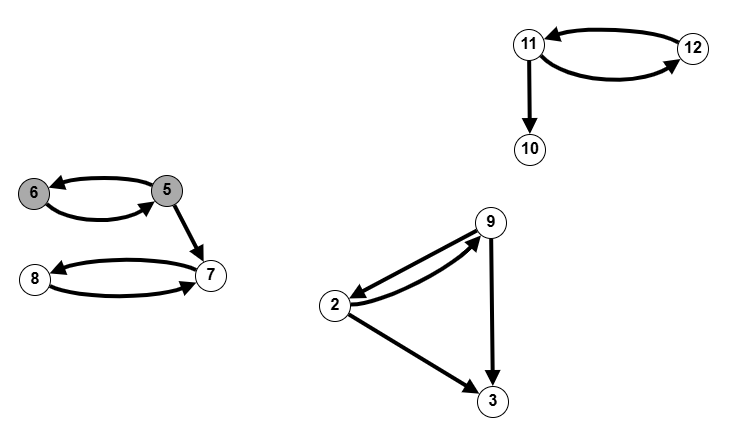
\includegraphics[width=\textwidth]{attachments/1/sk-2.png}
         \label{fig:1_1}
     \end{subfigure}
     \hfill
     \begin{subfigure}[t]{0.4\textwidth}
         \centering
         \caption*{\small{$x_0 := 7$\\
            $R(7)=\{7,8\}$\qquad$Q(7)=\{7,8\}$\qquad
            $\text{СК}(7) = \{7,8\}$}}
         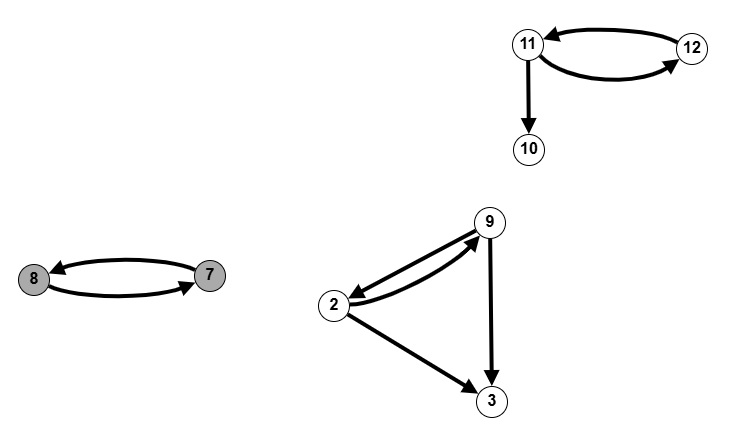
\includegraphics[width=\textwidth]{attachments/1/sk-3.png}
         \label{fig:1_2}
        \end{subfigure}
          \hfill
     \begin{subfigure}[t]{0.22\textwidth}
         \centering
         \caption*{\small{$x_0 := 2$\quad
        $R(2)=\{2,3,9\}$\\$Q(2)=\{2,9\}$\\
        $\text{СК}(2) = \{2,9\}$}}
         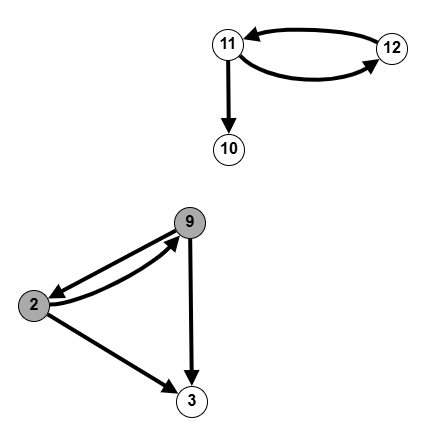
\includegraphics[width=\textwidth]{attachments/1/sk-4.png}
         \label{fig:1_3}
        \end{subfigure}
    \hfill
     \begin{subfigure}[t]{0.17\textwidth}
         \centering
         \caption*{\small{$x_0 := 11$\\
        $R(11)=\{10,11,12\}$\\$Q(11)=\{11,12\}$\\
        $\text{СК}(11) = \{11,12\}$}}
         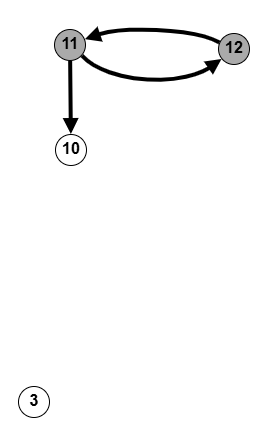
\includegraphics[width=\textwidth]{attachments/1/sk-5.png}
         \label{fig:1_4}
        \end{subfigure}
    \hfill
     \begin{subfigure}[t]{0.13\textwidth}
         \centering
         \caption*{\footnotesize{$\text{СК}(10)=\{10\},\\
         \text{СК}(3) = \{3\}$}}
         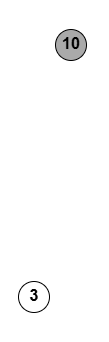
\includegraphics[width=0.7\textwidth]{attachments/1/sk-6.png}
         \label{fig:1_4}
        \end{subfigure}
    \caption{Выявление сильных компонент}
    \label{fig:1_sk}
\end{figure}
\end{enumerate}


\clearpage% 2------------------------------------------
\begin{enumerate} 
\item[\textbf{Задача 2.}] Крупный интернет-магазин ювелирных изделий для привлечения и удержания клиентов принял решение внедрить рекомендательную систему в своей системе электронного бизнеса. Рекомендательные системы строятся на основе технологии анализа клиентских сред. Профиль пользователя – это структура, выражающая предпочтения пользователя или группы пользователей на основе примеров. Если созданы профили пользователей, то в момент обращения какого-то клиента система подбирает похожие профили и, учитывая степень схожести, составляет рекомендации для клиента.\\
Пусть создается профиль сегмента VIP-клиентов интернет-магазина SerenaGold на основе предложений от «Бриллиантов Якутии», и построен граф предпочтений, представленный на рисунке. Вершины соответствуют предложениям, причем если предложение $i$ пользуется большим спросом, чем предложение $j$, то от $i$ к $j$ ведет дуга. Постройте последовательность предложений от «Бриллиантов Якутии», упорядоченную по убыванию
предпочтительности. \\

\begin{center}
Решение 
\end{center}
Разложим данный бесконтурный графа на уровни методом вычеркивания дуг, как представлено на рисунке \ref{fig:2_lvls}.\\
\begin{figure}[ht]
     \centering
     \begin{subfigure}[b]{0.3\textwidth}
        \centering
         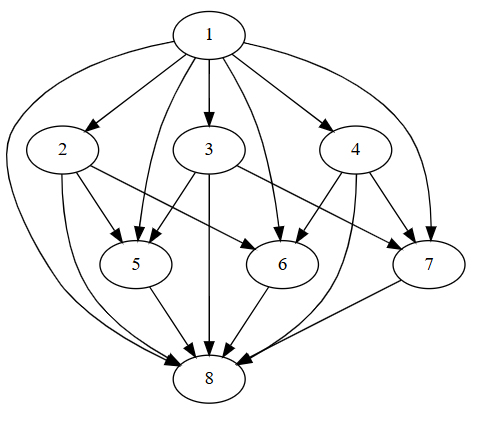
\includegraphics[width=\textwidth]{attachments/2/0.png}
         \caption*{\small{Вершина без входящих дуг: вершина 1}}
         \label{fig:2_0}
     \end{subfigure}
     \hfill
     \begin{subfigure}[b]{0.25\textwidth}
        \centering
         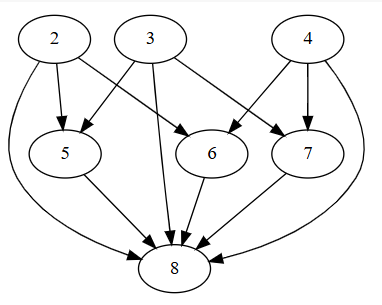
\includegraphics[width=\textwidth]{attachments/2/1.png}
         \caption*{\small{Вершины без входящих дуг: вершины 2,3,4}}
         \label{fig:2_1}
     \end{subfigure}
     \hfill
     \begin{subfigure}[b]{0.20\textwidth}
         \centering
         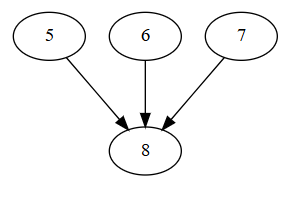
\includegraphics[width=\textwidth]{attachments/2/2.png}
         \caption*{\small{Вершины без входящих дуг: вершины 5,6,7}}
         \label{fig:2_2}
        \end{subfigure}
    \hfill
     \begin{subfigure}[b]{0.1\textwidth}
         \centering
         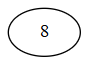
\includegraphics[width=0.6\textwidth]{attachments/2/3.png}
         \caption*{\small{Одна вершина 8}}
         \label{fig:2_3}
     \end{subfigure}
    \caption{Метод вычеркивания дуг}
    \label{fig:2_lvls}
\end{figure}
\begin{table}[ht]
    \centering
    \begin{tabular}{c|c}
    \hline
    \textit{Уровень} & \textit{Вершины} \\ \hline
    1 & 1 \\
    2 & 2,3,4 \\
    3 & 5,6,7 \\
    4 & 8 \\ \hline
    \end{tabular}
    \caption{Соответствие вершин уровням}
    \label{tab:2_lvls}
\end{table}\\
Таким образом, последовательность предложений от «Бриллиантов Якутии», упорядоченная по убыванию
предпочтительности, согласно разложению по уровням имеет вид:\\
1, 2 или 3 или 4, 5 или 6 или 7, 8. 
\end{enumerate}


\clearpage% 3------------------------------------------
\begin{enumerate}
\item[\textbf{Задача 3.}] Пусть задана последовательность целых чисел $(5,4,4,4,3,3,3,2)$. Является ли данная последовательность графической и для какого графа (связный, гамильтонов, дерево)? Если ответ положительный, то на основе приведенных в лекции критериев с помощью $d$-процедуры построить соответствующий
граф.\\ 
\begin{center}
Решение 
\end{center}
\textbf{Критерий для построения дерева:} последовательность степеней $(d_1, \dots, d_n)$ является последовательностью степеней дерева тогда и только тогда, когда $(d_i > 1)$, $\forall i = \overline{1,n}$ и $\sum_{i=1}^{n} d_i = 2 (n - 1)$, при этом на каждом шаге в качестве ведущей вершины следует выбирать вершину с минимальной положительной степенью.\\
В данном случае критерий \qquad $5+4\times3+3\times3+2 \neq 2 (8-1)$ \\
не выполняется: \qquad \qquad \qquad \quad$28 \neq 14$
\\
\\
\textbf{Критерий для построения связного графа :} правильная последовательность степеней $(d_1, \dots, d_n)$ может быть реализована связным графом тогда и только тогда, когда $(d_i > 1)$, $\forall i = \overline{1,n}$ и $\sum_{i=1}^{n} d_i \ge 2 (n - 1)$, при этом на каждом шаге в качестве ведущей вершины следует выбирать вершину с минимальной положительной степенью.\\
В данном случае критерий \qquad $5+4\times3+3\times3+2 \ge 2 (8-1)$ \\
выполняется: \qquad \qquad \qquad \qquad$28 \ge 14$
\\
\\
\textbf{Критерий для построения гамильтонова графа:} если существует графическая реализация правильной последовательности $(d_1, \dots, d_n)$ с гамильтоновым путем, проходящим через вершину степени $(d_j)$, то к такой реализации приведет $d-$процедура, на первом шаге которой выбирается вершина степени $(d_i > 1)$, а на каждом из последующих -- вершина с минимальной положительной остаточной степенью из множества $\Gamma(v)$, где $(v)$ -- ведущая вершина на предыдущем шаге.\\
\\
\\
Так как всякий гамильтонов граф является связным, для начала имеет смысл проверить, является ли заданная последовательность графической для гамильтонова графа. Процесс рассуждений представлен на рисунке \ref{fig:3_gamilton}.
\begin{figure}
     \centering
     \begin{subfigure}[b]{0.2\textwidth}
         \centering
         \caption*{\footnotesize{Изначально ни одна из вершин не соединена ни с одной другой}}
         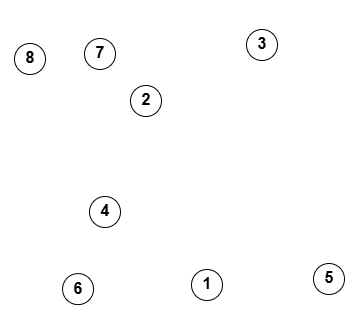
\includegraphics[width=\textwidth]{attachments/3/1.png}
         \label{fig:3_0}
     \end{subfigure}
     \hfill
     \begin{subfigure}[b]{0.2\textwidth}
         \centering
         \caption*{\footnotesize{Выберем произвольную вершину в качестве ведущей \quad\textemdash\quad $X_1$}}
         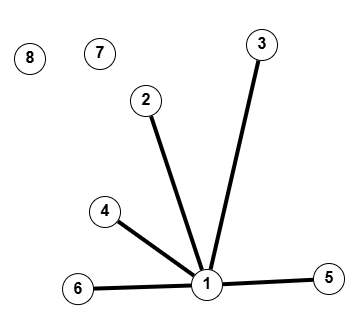
\includegraphics[width=\textwidth]{attachments/3/2.png}
         \label{fig:3_1}
     \end{subfigure}
     \hfill
     \begin{subfigure}[b]{0.2\textwidth}
         \centering
         \caption*{\footnotesize{$v = X_1$. Ведущей избираем $X_5 \in \Gamma(v)=\{X_2,X_3,X_4,X_5,X_6\}$,}}
         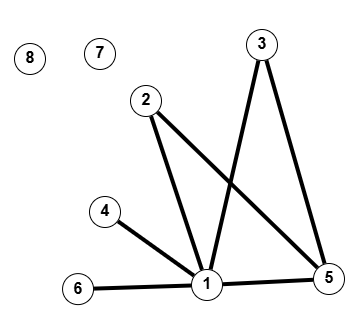
\includegraphics[width=\textwidth]{attachments/3/3.png}
         \label{fig:3_2}
     \end{subfigure}
     \hfill
     \begin{subfigure}[b]{0.2\textwidth}
         \centering
         \caption*{\footnotesize{$\Gamma(v) = \{X_2,X_3\}$,$v = X_5$. Ведущей избираем $X_3$}}
         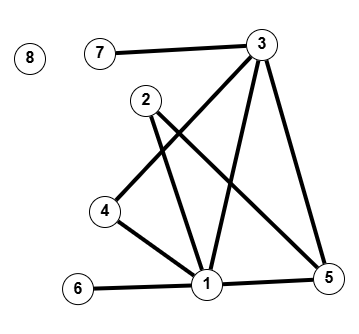
\includegraphics[width=\textwidth]{attachments/3/4.png}
         \label{fig:3_3}
     \end{subfigure}
     \hfill
     \begin{subfigure}[b]{0.2\textwidth}
         \centering
         \caption*{\footnotesize{$\Gamma(v) = \{X_4,X_7\}$,$v = X_3$. Ведущей избираем $X_4$}}
         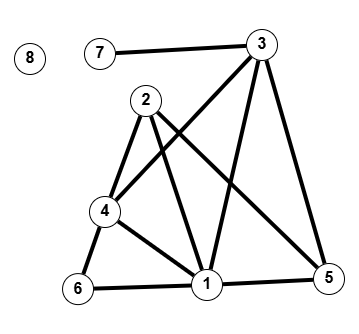
\includegraphics[width=\textwidth]{attachments/3/5.png}
         \label{fig:3_4}
     \end{subfigure}
     \hfill
     \begin{subfigure}[b]{0.2\textwidth}
         \centering
         \caption*{\footnotesize{$\Gamma(v) = \{X_2,X_6\}$,$v = X_4$. Ведущей избираем $X_2$}}
         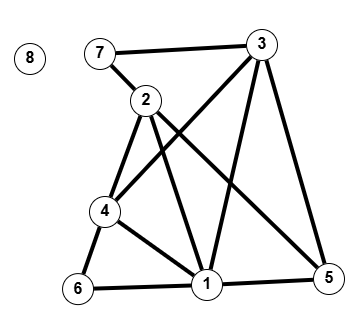
\includegraphics[width=\textwidth]{attachments/3/6.png}
         \label{fig:3_5}
     \end{subfigure}
     \hfill
     \begin{subfigure}[b]{0.2\textwidth}
         \centering
         \caption*{\footnotesize{$\Gamma(v) = \{X_7\}, v = X_2$. Ведущей избираем $X_7$}}
         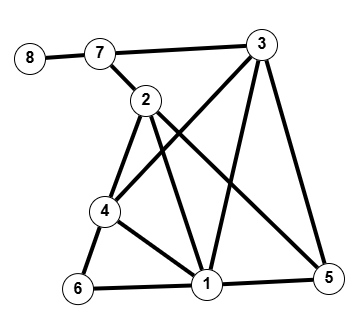
\includegraphics[width=\textwidth]{attachments/3/7.png}
         \label{fig:3_6}
     \end{subfigure}
     \hfill
     \begin{subfigure}[b]{0.2\textwidth}
         \centering
         \caption*{\footnotesize{$\Gamma(v) = \{X_8\}$,$v = X_7$. Ведущей избираем $X_8$}}
         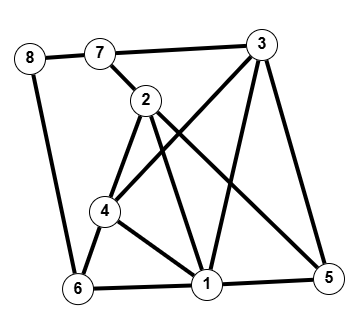
\includegraphics[width=\textwidth]{attachments/3/8.png}
         \label{fig:3_7}
     \end{subfigure}
        \caption{Процедура построения гамильтонова графа по заданной последовательности}
        \label{fig:3_gamilton}
\end{figure}
\begin{table}[!ht]
    \centering
    \begin{tabular}{|c|c|c|c|c|c|c|c|c|} \hline  
        \textit{0} & X1 & X2 & X3 & X4 & X5 & X6 & X7 &X8   \\ \hline 
        ~ & 5 & 4 & 4 & 4 & 3 & 3 & 3 &2 \\ \hline  
        ~ & 5& 4& 4& 4& 3& 3& 3 &2 \\ \hline 
        \textit{1} & \cellcolor{blue!25}X1 & X2 & X3 & X4 & X5 & X6 & X7 & X8 \\ \hline  
        & \cellcolor{blue!25}5 & 4 & 4 & 4 & 3 & 3 & 3 & 2 \\ \hline  
        & \cellcolor{blue!25}0 & 3 & 3 & 3 & 2 & 2 & 3 & 2 \\ \hline  
        \textit{2} & X2 & X3 & X4 & X7 & \cellcolor{blue!25}X5 & X6 & X8 & X1 \\ \hline  
        ~ & 3 & 3 & 3 & 3 & \cellcolor{blue!25}2 & 2 & 2 & 0 \\ \hline  
        ~ & 2 & 2 & 3 & 3 & \cellcolor{blue!25}0 & 2 & 2 & 0 \\ \hline  
        \textit{3} & X4 & X7 & X2 & \cellcolor{blue!25}X3 & X6 & X8 & X1 & X5 \\ \hline  
        ~ & 3 & 3 & 2 & \cellcolor{blue!25}2 & 2 & 2 & 0 & 0 \\ \hline  
        ~ & 2 & 2 & 2 & \cellcolor{blue!25}0 & 2 & 2 & 0 & 0 \\ \hline  
        \textit{4} & X2 & \cellcolor{blue!25}X4 & X6 & X7 & X8 & X1 & X5 & X3 \\ \hline  
        ~ & 2 & \cellcolor{blue!25}2 & 2 & 2 & 2 & 0 & 0 & 0 \\ \hline  
        ~ & 1 & \cellcolor{blue!25}0 & 1 & 2 & 2 & 0 & 0 & 0 \\ \hline  
        \textit{5} & X7 & X8 & \cellcolor{blue!25}X2 & X6 & X1 & X5 & X3 & X4 \\ \hline  
        ~ & 2 & 2 & \cellcolor{blue!25}1 & 1 & 0 & 0 & 0 & 0 \\ \hline  
        ~ & 1 & 2 & \cellcolor{blue!25}0 & 1 & 0 & 0 & 0 & 0 \\ \hline  
        \textit{6} & X8 & \cellcolor{blue!25}X7 & X6 & X1 & X5 & X3 & X2 & X4 \\ \hline  
        ~ & 2 & \cellcolor{blue!25}1 & 1 & 0 & 0 & 0 & 0 & 0 \\ \hline  
        ~ & 1 & \cellcolor{blue!25}0 & 1 & 0 & 0 & 0 & 0 & 0 \\ \hline  
        \textit{7} & \cellcolor{blue!25}X8 & X6 & X1 & X5 & X3 & X2 & X4 & X7 \\ \hline  
        ~ & \cellcolor{blue!25}1 & 1 & 0 & 0 & 0 & 0 & 0 & 0 \\ \hline  
        ~ & \cellcolor{blue!25}0 & 0 & 0 & 0 & 0 & 0 & 0 & 0 \\ \hline 
    \end{tabular}
    \caption{Таблица построения графа}
    \label{tab:3_table}
\end{table}
\\
\\
Граф был построен успешно, процедура дошла до критерия останова: $d_i = 0,\quad \forall i = \overline{1,n}$, что отражено в таблице \ref{tab:3_table}.
\\
При этом построенный граф действительно является гамильтоновым, так как в нем существует гамильтонов путь \quad\textemdash\quad простой цикл, в который входят все вершины графа; в данном случае, например:
 $[1,5,3,4,2,7,8,6]$.
\end{enumerate}


\clearpage% 4-----------------------------------
\begin{enumerate}\item[\textbf{Задача 4.}] Алгоритм нахождения максимальных независимых множеств приведен в книге "Теория графов. Алгоритмический подход" (Н. Кристофидес, стр. 46-49). Используя данный алгоритм, найдите максимальные независимые множества для графа, изображенного на рисунке \ref{fig:figure4_graph}. Проверьте правильность работы критерия останова.
\begin{figure}[h]
    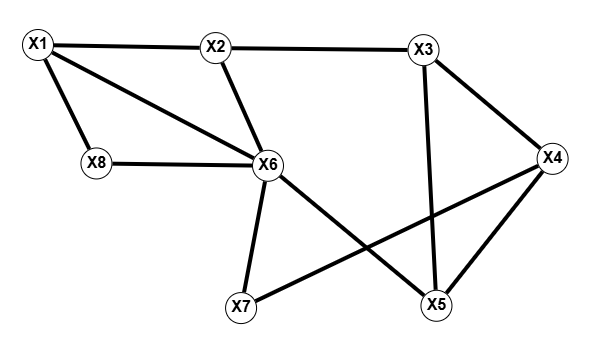
\includegraphics[width=0.45\textwidth, center]{attachments/4/graph.png}
    \caption{Граф для задачи 4}
    \label{fig:figure4_graph}
\end{figure}
\begin{center}
Решение 
\end{center}
\begin{enumerate}
    \item[0.] Инициализация:
        \quad $k = 0$
        \quad $S_0 = Q_0^{-} =\varnothing$,
        \quad  $Q_0^{+} = X = \{x_1,x_2,x_3,x_4,x_5,x_6,x_7,x_8\}$
    \item[1.] %Выберем произвольную вершину из множества доступных вершин  $Q_0^{+}$ \quad\textemdash \quad вершину $x_1$, тогда:\\\quad 
        $k = k +1 = 1$,
        \quad $S_1 = \{x_6\}$,
        \quad  $Q_1^{+} =Q_0^{+} \hspace{1mm}\backslash\hspace{1mm} (\Gamma (x_6) \cup x_6) = \{x_3,x_4\}$,
        \quad  $Q_1^{-} = \varnothing$
    \item[2.] $k = k+1 = 2$,
        \quad $S_2 = \{x_6,x_3\}$
        \quad  $Q_2^{+} =Q_1^{+} \hspace{1mm}\backslash\hspace{1mm} (\Gamma (x_3) \cup x_3) =  \varnothing$,
        \quad  $Q_2^{-} = \varnothing$\\
         $Q_2^{-} = Q_2^{+} = \varnothing\quad\Longrightarrow \textbf{Максимальное Независимое Множество: }\{x_3,x_6\}$.
    \item[3.]  $k = k - 1 = 1$,
        \quad $S_1 = \{x_6\}$,
        \quad  $Q_1^{+} =\{x_4\}$,
        \quad  $Q_1^{-} = \{x_3\}$
    \item[4.] $k = k + 1 = 2$,
        \quad $S_2 = \{x_6, x_4\}$,
        \quad  $Q_2^{+} =\varnothing$,
        \quad  $Q_2^{-} = \varnothing$\\
        $Q_2^{-} = Q_2^{+} = \varnothing\quad\Longrightarrow \textbf{Максимальное Независимое Множество: }\{x_4,x_6\}$.
    \item[5.] $k = k - 1 = 1$,
        \quad $S_1 = \{x_6\}$,
        \quad  $Q_1^{+} =\varnothing$,
        \quad  $Q_1^{-} = \{x_3,x_4\}$
    \item[6.] $k = k - 1 = 0$,
        \quad $S_0 =\varnothing$,
        \quad  $Q_0^{+} =\{x_1,x_2,x_3,x_4,x_5,x_7,x_8\}$,
        \quad  $Q_0^{-} = \{x_6\}$
    \item[7.] $k = k + 1 = 1$,
        \quad $S_1 =\{x_1\}$,
        \quad  $Q_1^{+} =\{x_3,x_4,x_5,x_7\}$,
        \quad  $Q_1^{-} = \varnothing$
    \item[8.] $k = k + 1 = 2$,
        \quad $S_2 =\{x_1, x_7\}$,
        \quad  $Q_2^{+} =\{x_3,x_5\}$,
        \quad  $Q_2^{-} = \varnothing$
    \item[9.] $k = k + 1 = 3$,
        \quad $S_3 =\{x_1,x_7, x_3\}$,
        \quad  $Q_3^{+} =\varnothing$,
        \quad  $Q_3^{-} = \varnothing$\\
        $Q_3^{-} = Q_3^{+} = \varnothing\quad\Longrightarrow \textbf{Максимальное Независимое Множество: }\{x_1, x_3,x_7\}$.
    \item[10.] $k = k - 1 = 2$,
        \quad $S_2 =\{x_1,x_7\}$,
        \quad  $Q_2^{+} =\{x_5\}$,
        \quad  $Q_2^{-} = \{x_3\}$
    \item[11.] $k = k + 1 = 3$,
        \quad $S_3 =\{x_1,x_7, x_5\}$,
        \quad  $Q_3^{+} =\varnothing$,
        \quad  $Q_3^{-} = \varnothing$\\
        $Q_3^{-} = Q_3^{+} = \varnothing\quad\Longrightarrow \textbf{Максимальное Независимое Множество: }\{x_1, x_5,x_7\}$.
    \item[12.] $k = k - 1 = 2$,
        \quad $S_2 =\{x_1,x_7\}$,
        \quad  $Q_2^{+} =\varnothing$,
        \quad  $Q_2^{-} = \{x_3,x_5\}$
    \item[13.] $k = k - 1 = 1$,
        \quad $S_1 =\{x_1\}$,
        \quad  $Q_1^{+} =\{x_4\}$,
        \quad  $Q_1^{-} = \{x_3,x_5,x_7\}$
    \item[14.] $k = k + 1 = 2$,
        \quad $S_2 =\{x_1,x_4\}$,
        \quad  $Q_2^{+} =\varnothing$,
        \quad  $Q_2^{-} = \varnothing$\\
        $Q_2^{-} = Q_2^{+} = \varnothing \Longrightarrow \textbf{Максимальное Независимое Множество: }\{x_1, x_4\}$.
    \item[15.] $k = k - 1 = 1$,
        \quad $S_1 =\{x_1\}$,
        \quad  $Q_1^{+} =\varnothing$,
        \quad  $Q_1^{-} = \{x_3,x_4,x_5,x_7\}$
    \item[16.] $k = k - 1 = 0$,
        \quad $S_0 =\varnothing$,
        \quad  $Q_0^{+} =\{x_2,x_3,x_4,x_5,x_7,x_8\}$,
        \quad  $Q_0^{-} = \{x_1,x_6\}$
    \item[17.] $k = k + 1 = 1$,
        \quad $S_1 =\{x_8\}$,
        \quad  $Q_1^{+} =\{x_2,x_3,x_4,x_5,x_7\}$,
        \quad  $Q_1^{-} = \varnothing$
    \item[18.] $k = k + 1 = 2$,
        \quad $S_2 =\{x_8, x_2\}$,
        \quad  $Q_2^{+} =\{x_4,x_5,x_7\}$,
        \quad  $Q_2^{-} = \varnothing$
    \item[19.] $k = k + 1 = 3$,
        \quad $S_3 =\{x_8,x_2, x_4\}$,
        \quad  $Q_3^{+} =\varnothing$,
        \quad  $Q_3^{-} = \varnothing$\\
        $Q_3^{-} = Q_3^{+} = \varnothing\quad\Longrightarrow \textbf{Максимальное Независимое Множество: }\{x_2, x_4,x_8\}$.
    \item[20.] $k = k - 1 = 2$,
        \quad $S_2 =\{x_8,x_2\}$,
        \quad  $Q_2^{+} =\{x_5,x_7\}$,
        \quad  $Q_2^{-} = \{x_4\}$
    \item[21.] $k = k + 1 = 3$,
        \quad $S_3 =\{x_8,x_2, x_5\}$,
        \quad  $Q_3^{+} =\{x_7\}$,
        \quad  $Q_3^{-} = \varnothing$
    \item[22.] $k = k + 1 = 4$,
        \quad $S_4 =\{x_8,x_2, x_5,x_7\}$,
        \quad  $Q_4^{+} =\varnothing$,
        \quad  $Q_4^{-} = \varnothing$\\
        $Q_4^{-} = Q_4^{+} = \varnothing\qquad\Longrightarrow \textbf{Максимальное Независимое Множество: }\{x_2, x_5,x_7,x_8\}$.
    \item[23.] $k = k - 1 = 3$,
        \quad $S_3 =\{x_8,x_2, x_5\}$,
        \quad  $Q_3^{+} =\varnothing$,
        \quad  $Q_3^{-} = \{x_7\}$
    \item[24.] $k = k - 1 = 2$,
        \quad $S_2 =\{x_8,x_2\}$,
        \quad  $Q_2^{+} =\varnothing$,
        \quad  $Q_2^{-} = \{x_4,x_5,x_7\}$
    \item[25.] $k = k - 1 = 1$,
        \quad $S_1 =\{x_8\}$,
        \quad  $Q_1^{+} =\{x_3,x_4,x_5,x_7\}$,
        \quad  $Q_1^{-} = \{x_2\}$
    \item[26.] $k = k + 1 = 2$,
        \quad $S_2 =\{x_8, x_3\}$,
        \quad  $Q_2^{+} =\{x_7\}$,
        \quad  $Q_2^{-} = \varnothing$
    \item[27.] $k = k + 1 = 3$,
        \quad $S_3 =\{x_8,x_3, x_7\}$,
        \quad  $Q_3^{+} =\varnothing$,
        \quad  $Q_3^{-} = \varnothing$\\
        $Q_3^{-} = Q_3^{+} = \varnothing\quad\Longrightarrow \textbf{Максимальное Независимое Множество: }\{x_3, x_7,x_8\}$.
     \item[28.] $k = k - 1 = 2$,
        \quad $S_2 =\{x_8,x_3\}$,
        \quad  $Q_2^{+} =\varnothing$,
        \quad  $Q_2^{-} = \{x_7\}$
     \item[29.] $k = k - 1 = 1$,
        \quad $S_1 =\{x_8\}$,
        \quad  $Q_1^{+} =\{x_4,x_5,x_7\}$,
        \quad  $Q_1^{-} = \{x_2,x_3\}$
    \item[30.] $k = k + 1 =2$,
        \quad $S_2 =\{x_8,x_5\}$,
        \quad  $Q_2^{+} =\{x_7\}$,
        \quad  $Q_2^{-} = \{x_2\}$\\
    $\exists x_2 \in Q_2^{-}: \Gamma (x_2) \cap Q_2^{+} = \varnothing\quad\Longrightarrow$ переходим к шагу возвращения.
    \item[31.] $k = k - 1 =1$,
        \quad $S_1 =\{x_8\}$,
        \quad  $Q_1^{+} =\{x_4,x_7\}$,
        \quad  $Q_1^{-} = \{x_2,x_3,x_5\}$
    \item[32.] $k = k + 1 =2$,
        \quad $S_2 =\{x_8,x_4\}$,
        \quad  $Q_2^{+} =\varnothing$,
        \quad  $Q_2^{-} = \{x_2\}$\\
    $Q_2^{+}=\varnothing\text{ и }Q_2^{-} \neq\varnothing\quad\Longrightarrow$ переходим к шагу возвращения.
    \item[32.] $k = k - 1 = 1$,
        \quad $S_1 =\{x_8\}$,
        \quad  $Q_1^{+} =\{x_7\}$,
        \quad  $Q_1^{-} = \{x_2,x_3,x_4,x_5\}$\\
    $\exists x_2 \in Q_1^{-}: \Gamma (x_2) \cap Q_1^{+} = \varnothing\quad\Longrightarrow$ переходим к шагу возвращения.
    \item[33.] $k = k - 1 = 0$,
        \quad $S_0 =\varnothing$,
        \quad  $Q_0^{+} =\{x_2,x_3,x_4,x_5,x_7\}$,
        \quad  $Q_0^{-} = \{x_1,x_6,x_8\}$\\
    $\exists x_8 \in Q_0^{-}: \Gamma (x_8) \cap Q_0  ^{+} = \varnothing\quad\Longrightarrow$ переходим к шагу возвращения, \textbf{\textit{НО}} $k = k - 1 = -1$.
    \\
\end{enumerate}
{\color{blue} Можем сделать вывод, что критерий останова не выполняется корректно в некоторых случаях, а именно - если в множестве уже использованных вершин $Q_0^{-}$ есть такая вершина, что каждая из смежных ей вершин уже использована, иначе говоря: удовлетворяется условие (3.8) из книги, что ведет к шагу возвращения, однако возвращение невозможно, так как $k = 0$ уже. Возможная модификация:
для удовлетворения критерия останова, который предполагает, что $k = 0$ и $Q_0^{+}=\varnothing$:
если на шаге 3 удовлетворяется условие и $k = 0$, то не имеет смысла прибегать к шагу возвращения, то есть к шагу 5, сразу переходить к шагу 2, чтобы перебрать оставшиеся вершины и дойти до требуемого $Q_0^{+}=\varnothing$.}
\begin{figure}[h]
    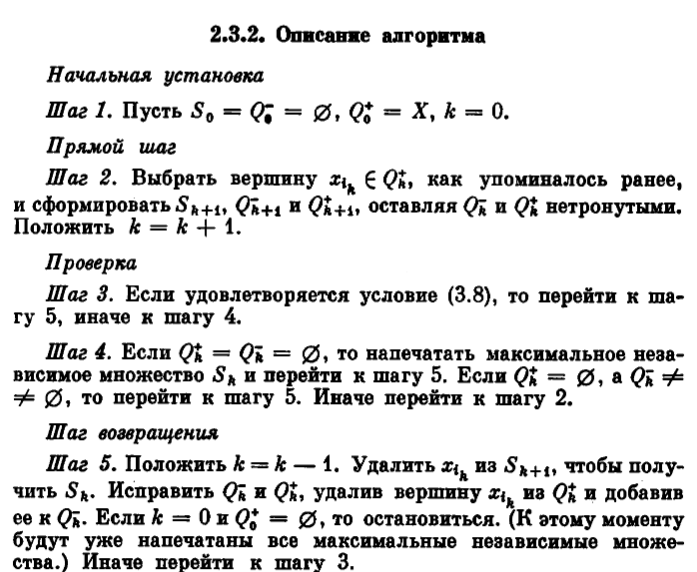
\includegraphics[width=0.4\textwidth, center]{attachments/4/algo.png}
    \caption{Алгоритм}
    \label{fig:figure4_algo}
\end{figure}

\end{enumerate}


\clearpage% 5-----------------------------------
\begin{enumerate}
\item[\textbf{Задача 5.}] Найти ядро графа, представленного матрицей смежности на рисунке \ref{fig:5_adj_matrix}.
\begin{figure}[ht]
  \begin{minipage}[b]{0.5\textwidth}
    \centering
    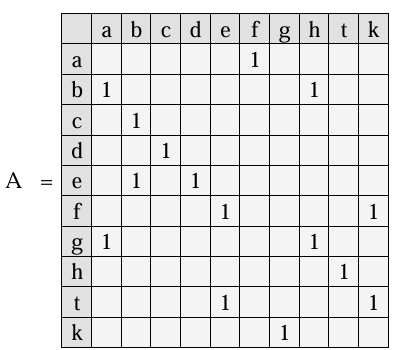
\includegraphics[width=0.8\textwidth, center]{attachments/5/matrix.png}
    \caption{Матрица смежности}
    \label{fig:5_adj_matrix}
  \end{minipage}
  \hfill
  \begin{minipage}[b]{0.5\textwidth}
    \centering
    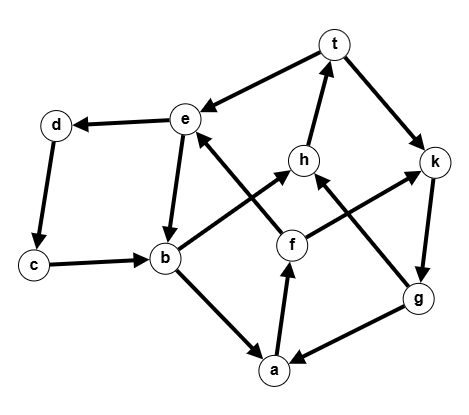
\includegraphics[width=.75\textwidth, center]{attachments/5/graph.png}
    \caption{Граф $G$}
    \label{fig:5_graph}
  \end{minipage}
\end{figure}
\begin{center}
Решение 
\end{center}
Изобразим граф $G$, соответствующий заданной матрице смежности $A$, на рисунке \ref{fig:5_graph}. 

Разобьем множество вершин графа на два подмножества: $X_1 = \{a, c, e, h, k\}$ и $X_2 = \{b,d,f,g,t\}$.
Заметим, что $X_1 \cap X_2 = \varnothing$, $X_1 \cup X_2 = X$ и для каждой из дуг графа верно, что одна концевая вершина принадлежит $X_1$ и другая - $X_2$. Следовательно, граф $G$ \quad\textemdash\quad двудольный граф, что наглядно показано на рисунке \ref{fig:5_bigraph}.
В двудольном графе все контуры имеют чётную длину, так как для построения контура необходимо чередование дуг из двух долей.
Следовательно, граф $G$ \quad\textemdash\quad граф без нечетных контуров.\\
Орграф является сильно связным, если для любой пары вершин $x_i,x_j$ в графе существует путь из $x_i$ в $x_j$ и из $x_j$ в $x_i$. Заметим, что $G$ \quad\textemdash\quad сильно связный орграф.
\begin{figure}[h]
    \centering
    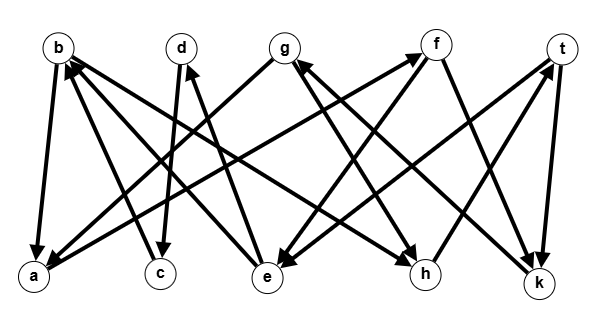
\includegraphics[width=0.5\textwidth, center]{attachments/5/bigraph.png}
    \caption{Граф $G$}
    \label{fig:5_bigraph}
\end{figure}
\\
\\
Таким образом, в графе $G$ как в сильно связном графе без нечетких контуров существует 2 ядра, для нахождения которых воспользуемся алгоритмом:\\
\begin{enumerate}
    \item[\textbf{S1}] Выберем произвольную вершину $x_0$. В ядро $Y_1$ включим выбранную вершину $x_0$ и все вершины, достижимые из $x_0$ с помощью простого пути четной длины.\\
    $x_0 = F$\\$Y_1=\{b,d,f,g,t\}$
    \item[\textbf{S2}] Положим $Y_2 = X \backslash Y_1$.\\
    $Y_2 = \{a, c, e, h, k\}$
\end{enumerate}
Выделенные ядра представлены на рисунке \ref{fig:5_ys}.
\begin{figure}[h]
    \centering
    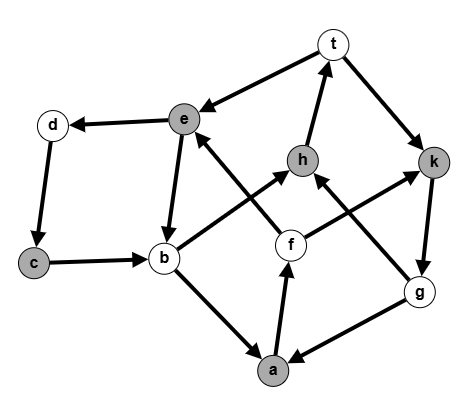
\includegraphics[width=0.5\textwidth, center]{attachments/5/res.png}
    \caption{Ядра графа $G$}
    \label{fig:5_ys}
\end{figure}
\end{enumerate}


%\clearpage% 6-------------
\begin{enumerate}
\item[\textbf{Задача 6.}] Предположим, что имеется квадратная таблица, состоящая из 16 ячеек. Ячейка контролирует себя и соседние, граничащие с ней ячейки. Определите наименьшее возможное число контролирующих ячеек и места их расположения в таблице, чтобы был обеспечен контроль всех ячеек таблицы.
\\
\begin{center}
Решение 
\end{center}
\begin{figure}[ht]
  \begin{minipage}[b]{0.5\textwidth}
    \centering
    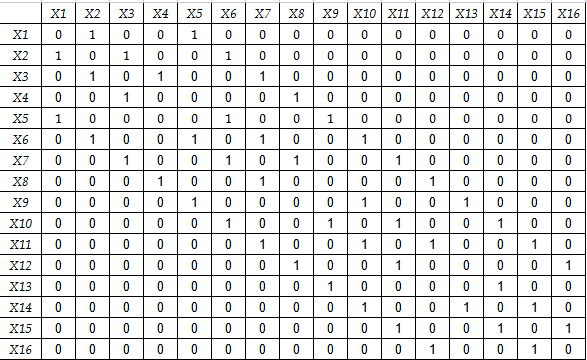
\includegraphics[width=\textwidth, center]{attachments/6/matrix.png}
    \caption{Матрица смежности}
    \label{fig:6_adj_matrix}
  \end{minipage}
  \hfill
  \begin{minipage}[b]{0.5\textwidth}
    \centering
    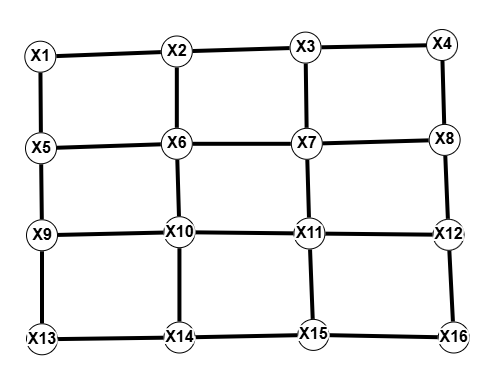
\includegraphics[width=.8\textwidth, center]{attachments/6/graph.png}
    \caption{Неорграф $G$}
    \label{fig:6_graph}
  \end{minipage}
\end{figure}
Построим неорграф $G = (X,U)$, множество вершин которого составляют 16 ячеек, множество дуг - соединения каждой из вершин с соответствующими соседними. Построенный неорграф изображен на рисунке \ref{fig:6_graph}. Тогда задача сводится к нахождению внешне устойчивого или доминирующего подмножества, то есть такого подмножества $D \subset X$, что для всякой вершины $x \in X, x \not\in D$ найдется такая вершина $y \in D$, что $y \rightarrow x$.
В неорграфе каждое максимальное независимое множество является доминирующим и, соответственно, ядром. Следовательно, для нахождения МНМ или МДМ применим алгоритм Магу со следующими модификациями:
\begin{align}
   &\Phi_{\text{ядро}}(x_1, \cdots, x_n) = \bigwedge_{i=1}^{n-1} \left( x_i \lor \left( \bigwedge_{\{(i, j):\atop a_{ij} = 1, j > i\}} x_j \right) \right) \\
    &\Phi_{\text{ядро}} = \bigvee_{r=1}^p K_r\text{, где }K_r\text{ — элементарная конъюнкция.}\\
    &\text{Для каждого }r = \overline{1, p} \text{ найти множества } Y_r = \{j : x_j \not\in K_r\}
\end{align}
Соответственно,
\begin{equation*}
\begin{aligned}
\Phi_{\text{ядро}} =
 & (x_1 \lor (x_2 \land x_5))
(x_2 \lor (x_3 \land x_6))
(x_3 \lor (x_4 \land x_7))
(x_4 \lor x_8) \\
 & (x_5 \lor (x_6 \land x_9))
(x_6 \lor (x_7 \land x_{10}))
(x_7 \lor (x_8 \land x_{11}))
(x_8 \lor x_{12}) \\
 & (x_9 \lor (x_{10} \land x_{13}))
(x_{10} \lor (x_{11} \land x_{14}))
(x_{11} \lor (x_{12} \land x_{15})) \\
 & (x_{12} \lor (x_{16})
(x_{13} \lor x_{14})
(x_{14} \lor x_{15})
(x_{15} \lor x_{16})
\end{aligned}
\end{equation*}
Программными средствами при помощи библиотеки sympy были проведены вычисления, дополненные скриптом выделения неупомянутых вершин, то есть требуемых для задачи МДМ.

Таким образом, мы получили два минимальных доминирующих множества: $K_1 = \{x8, x2, x9, x15\}$ и $K_2 = \{x5, x3, x14, x12\}$, отображенных на рисунке \ref{fig:6_mdm}.
\begin{figure}[ht]
  \begin{minipage}[b]{.5\linewidth}
    \centering
    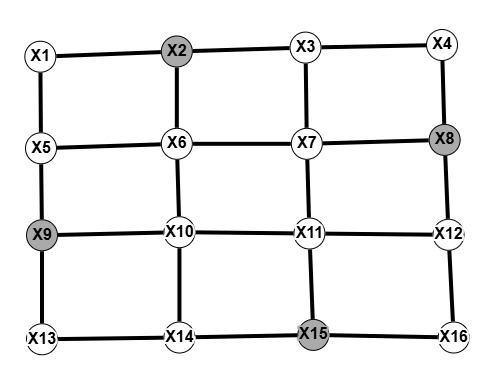
\includegraphics[width=\textwidth, center]{attachments/6/0.png}
  \end{minipage}
  \hfill
  \begin{minipage}[b]{.5\linewidth}
    \centering
    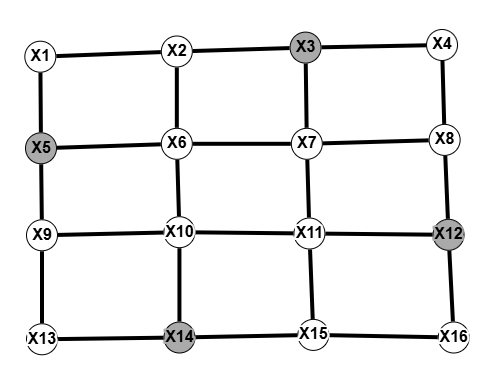
\includegraphics[width=\textwidth, center]{attachments/6/1.png}
  \end{minipage}
  \caption{Выявленные минимальные доминирующие множества}
  \label{fig:6_mdm}
\end{figure}
\begin{equation*}
\begin{aligned}
\Phi_{\text{ядро}} = & (x1 \land x11 \land x14 \land x16 \land x3 \land x6 \land x8 \land x9) \lor \\
& (x10 \land x12 \land x13 \land x15 \land x2 \land x4 \land x5 \land x7) \lor \\ & (x1 \land x11 \land x12 \land x14 \land x15 \land x3 \land x6 \land x8 \land x9) \lor \\ & (x10 \land x12 \land x13 \land x15 \land x2 \land x3 \land x5 \land x7 \land x8) \lor \\ & (x10 \land x12 \land x14 \land x15 \land x2 \land x4 \land x5 \land x7 \land x9) \lor \\ & (x11 \land x14 \land x16 \land x2 \land x3 \land x5 \land x6 \land x8 \land x9) \lor \\ & (x1 \land x10 \land x11 \land x12 \land x13 \land x15 \land x3 \land x5 \land x6 \land x8) \lor \\ & (x1 \land x10 \land x11 \land x12 \land x13 \land x15 \land x3 \land x6 \land x8 \land x9) \lor \\ & (x1 \land x10 \land x11 \land x13 \land x14 \land x16 \land x3 \land x5 \land x6 \land x8) \lor \\ & (x1 \land x10 \land x11 \land x13 \land x15 \land x16 \land x3 \land x5 \land x6 \land x8) \lor \\ & (x1 \land x10 \land x11 \land x13 \land x15 \land x16 \land x3 \land x6 \land x8 \land x9) \lor \\ & (x1 \land x10 \land x12 \land x13 \land x15 \land x2 \land x4 \land x6 \land x7 \land x9) \lor \\ & (x1 \land x10 \land x12 \land x13 \land x15 \land x3 \land x4 \land x5 \land x6 \land x7) \lor \\ & (x1 \land x10 \land x12 \land x13 \land x15 \land x3 \land x4 \land x6 \land x7 \land x9) \lor \\ & (x1 \land x10 \land x12 \land x13 \land x15 \land x3 \land x5 \land x6 \land x7 \land x8) \lor \\ & (x1 \land x10 \land x12 \land x13 \land x15 \land x3 \land x6 \land x7 \land x8 \land x9) \lor \\ & (x1 \land x10 \land x12 \land x14 \land x15 \land x2 \land x4 \land x6 \land x7 \land x9) \lor \\ & (x1 \land x10 \land x12 \land x14 \land x15 \land x3 \land x4 \land x6 \land x7 \land x9) \lor \\ & (x1 \land x10 \land x12 \land x14 \land x15 \land x3 \land x6 \land x7 \land x8 \land x9) \lor \\ & (x1 \land x11 \land x12 \land x14 \land x15 \land x2 \land x4 \land x6 \land x7 \land x9) \lor \\ & (x1 \land x11 \land x12 \land x14 \land x15 \land x3 \land x4 \land x6 \land x7 \land x9) \lor \\ & (x1 \land x11 \land x12 \land x14 \land x16 \land x2 \land x4 \land x6 \land x7 \land x9) \lor \\ & (x1 \land x11 \land x12 \land x14 \land x16 \land x3 \land x4 \land x6 \land x7 \land x9) \lor \\ & (x1 \land x11 \land x14 \land x16 \land x2 \land x4 \land x6 \land x7 \land x8 \land x9) \lor \\ & (x10 \land x11 \land x12 \land x13 \land x14 \land x16 \land x2 \land x4 \land x5 \land x7) \lor \\ & (x10 \land x11 \land x12 \land x13 \land x15 \land x2 \land x3 \land x5 \land x6 \land x8) \lor \\ & (x10 \land x11 \land x12 \land x14 \land x16 \land x2 \land x4 \land x5 \land x7 \land x9) \lor \\ & (x10 \land x11 \land x13 \land x14 \land x16 \land x2 \land x3 \land x5 \land x6 \land x8) \lor \\ & (x10 \land x11 \land x13 \land x14 \land x16 \land x2 \land x3 \land x5 \land x7 \land x8) \lor \\ & (x10 \land x11 \land x13 \land x14 \land x16 \land x2 \land x4 \land x5 \land x7 \land x8) \lor \\ & (x10 \land x11 \land x13 \land x15 \land x16 \land x2 \land x3 \land x5 \land x6 \land x8) \lor \\ & (x10 \land x11 \land x13 \land x15 \land x16 \land x2 \land x3 \land x5 \land x7 \land x8) \lor \\ & (x10 \land x11 \land x13 \land x15 \land x16 \land x2 \land x4 \land x5 \land x7 \land x8) \lor \\ & (x10 \land x11 \land x14 \land x16 \land x2 \land x3 \land x5 \land x7 \land x8 \land x9) \lor \\ & (x10 \land x11 \land x14 \land x16 \land x2 \land x4 \land x5 \land x7 \land x8 \land x9) \lor \\ & (x10 \land x12 \land x14 \land x15 \land x2 \land x3 \land x5 \land x7 \land x8 \land x9) \lor \\ & (x11 \land x12 \land x14 \land x15 \land x2 \land x3 \land x5 \land x6 \land x8 \land x9) \lor \\ & (x11 \land x12 \land x14 \land x15 \land x2 \land x4 \land x5 \land x6 \land x7 \land x9) \lor \\ & (x11 \land x12 \land x14 \land x16 \land x2 \land x4 \land x5 \land x6 \land x7 \land x9) \lor \\ & (x11 \land x14 \land x16 \land x2 \land x4 \land x5 \land x6 \land x7 \land x8 \land x9) \lor \\ & (x1 \land x10 \land x11 \land x12 \land x13 \land x14 \land x16 \land x3 \land x4 \land x5 \land x6 \land x7) \lor \\ & (x1 \land x10 \land x11 \land x13 \land x15 \land x16 \land x2 \land x4 \land x6 \land x7 \land x8 \land x9)
\end{aligned}
\end{equation*}
\end{enumerate}

\clearpage% 7----------------------------------------
\begin{enumerate}
\item[\textbf{Задача 7.}] На рисунке \ref{fig:7_graph} представлена схема, в которой вершины соответствуют клеммам, а ребра\quad\textemdash\quad прямым металлическим полоскам проводников. Для физически осуществимых соединений проводники не должны пересекаться, поэтому их нужно распределить по нескольким параллельным платам, учитывая, что клеммы «доступны» на всех платах. Определите минимальное число плат для реализации этих соединений.
\begin{figure}[ht]
    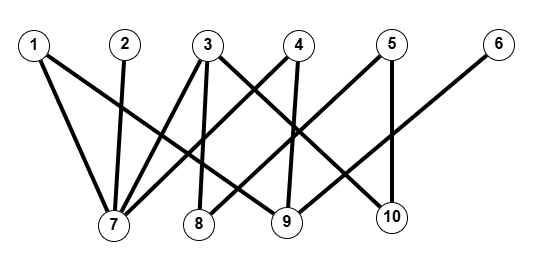
\includegraphics[width=0.5\textwidth, center]{attachments/7/0.png}
    \caption{Граф для задачи 7}
    \label{fig:7_graph}
\end{figure}
\begin{center}
Решение 
\end{center}
Для решения задачи используем алгоритм раскраски ребер, приняв за номер цвета\quad\textemdash\quad номер платы, так как ребра, соответствующие проводникам, не должны пересекаться, то есть быть на одной и той же плате. Используем последовательный метод раскраски: каждому ребру поставим в соответствие минимальный из номеров плат, неиспользуемых ребрами, смежными данному.\\
Таким образом, как представлено на рисунке \ref{fig:7_colours}, минимальное число плат\quad\textemdash\quad $4$ и распределение проводников по платам:
\begin{enumerate}
            \item[\textit{1 плата}]: 1-7, 3-8, 6-10
            \item[\textit{2 плата}]: 1-9, 2-7, 3-10, 6-8
            \item[\textit{3 плата}]: 6-9, 3-7
            \item[\textit{4 плата}]: 4-7
\end{enumerate}
\begin{figure}[ht]
  \begin{minipage}[b]{.5\linewidth}
    \centering
    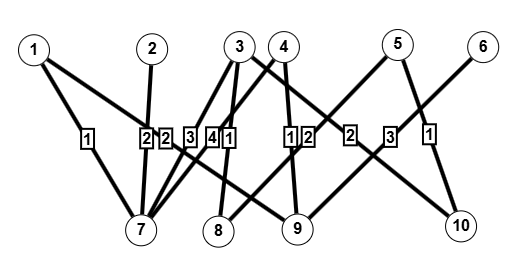
\includegraphics[width=\textwidth, center]{attachments/7/1.png}
  \end{minipage}
  \hfill
  \begin{minipage}[b]{.5\linewidth}
    \centering
    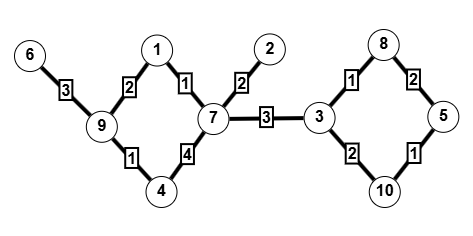
\includegraphics[width=\textwidth, center]{attachments/7/3.png}
  \end{minipage}
  \caption{Раскраска графа}
  \label{fig:7_colours}
\end{figure}
\end{enumerate}


\clearpage% 8 ------------------------------------------
\begin{enumerate}
\item[\textbf{Задача 8.}] На рисунке \ref{fig:8_graph} представлен граф, отражающий каналы связи между членами некоторой группы (каждой передаче сообщения от $i$ к $j$ приписана вероятность утечки информации). Требуется определить такой способ передачи конфиденциального сообщения между членами группы, при котором вероятность утечки информации будет наименьшей.
\\
% \begin{figure}[ht]
%     \centering
%     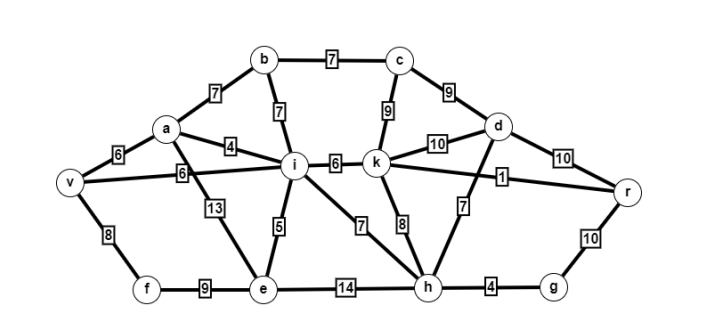
\includegraphics[width=0.9\textwidth, center]{attachments/8/0.png}
%     \caption{Каналы связи между членами группы}
%     \label{fig:8_graph}
% \end{figure}
\begin{figure}[ht]
  \begin{minipage}[b]{0.5\textwidth}
    \centering
    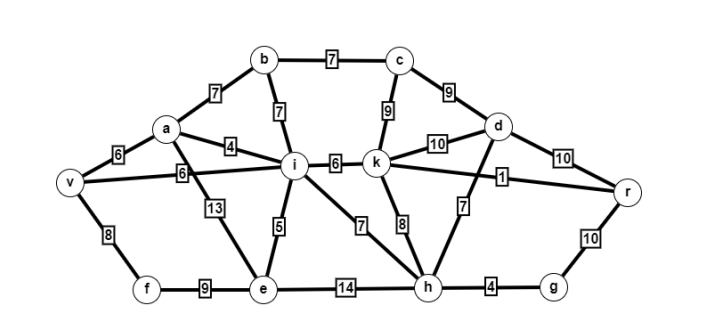
\includegraphics[width=\textwidth, center]{attachments/8/0.png}
    \caption{Каналы связи между членами группы}
    \label{fig:8_graph}
  \end{minipage}
  \hfill
  \begin{minipage}[b]{.5\textwidth}
    \centering
    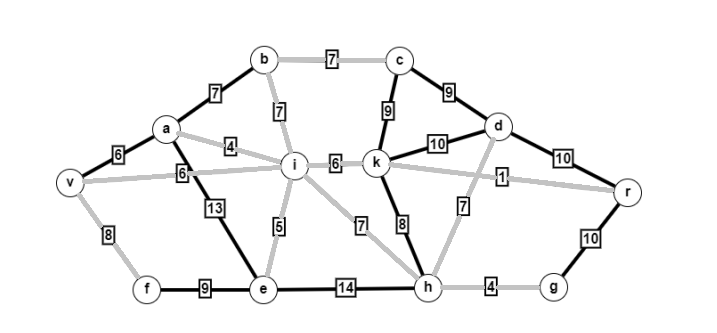
\includegraphics[width=\textwidth, center]{attachments/8/3.png}
        \caption{Выделенный способ передачи сообщения}
    \label{fig:8_ostov}
  \end{minipage}
\end{figure}
\begin{center}
Решение 
\end{center}
Требуется определить такой способ передачи конфиденциального сообщения между членами группы, при котором вероятность утечки информации будет наименьшей, то есть необходимо определить \textbf{остов наименьшего веса}, так как информация должна быть сообщена всем членам группы - все вершины должны быть включены - и суммарный вес - вероятность утечки информации - должен быть минимальным.\\
\\
Для нахождения остова минимального веса воспользуемся алгоритмом Прима; итерации отражены в таблице на рисунке \ref{fig:8_matrix}, при этом цветом выделена метка, выбранной на данном шаге вершины, и жирным шрифтом выделены метки смежных ей вершин.
\begin{figure}[h]
    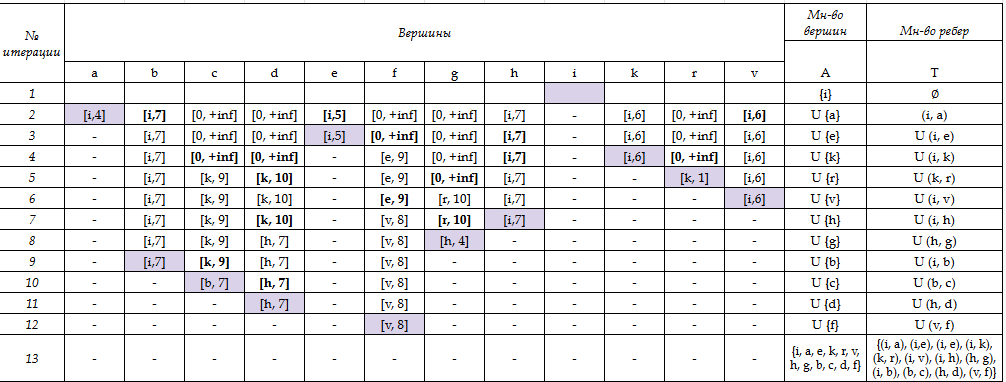
\includegraphics[width=\textwidth, center]{attachments/8/1.png}
    \caption{Таблица итераций алгоритма Прима}
    \label{fig:8_matrix}
\end{figure}
\\
Таким образом, наименьшая вероятность утечки информации составляет
$$4+5+6+1+6+7+4+7+7+7+8 = 62$$
и соответствующий способ передачи информации представлен на рисунке \ref{fig:8_ostov}.
\end{enumerate}


\clearpage% 9------------------------------------------
\begin{enumerate} 
\item[\textbf{Задача 9.}]IT-компания получила заказы на реализацию нескольких проектов, причем каждый проект может быть реализован за одно и то же время с привлечением некоторого подмножества ресурсов из множества ресурсов, имеющихся в наличии. Понятие ресурса понимается в широком смысле (разработчики, обладающие теми или иными компетенциями; компьютеры определенной мощности; некоторые приложения и программные среды и т.п.). В таблице на рисунке \ref{fig:9_table} представлены проекты и список ресурсов. Для каждого проекта символом «+» отмечены те ресурсы, которые используются при его реализации.
Укажите те проекты, которые можно выполнять одновременно за отведенный
промежуток времени в предположении, что все проекты начинаются в один и тот же момент времени.
\begin{figure}[ht]
  \begin{minipage}[b]{0.65\textwidth}
    \centering
    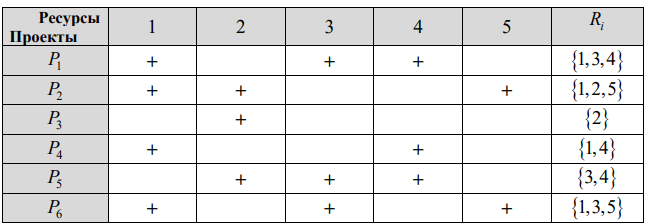
\includegraphics[width=\textwidth, center]{attachments/9/0.png}
    \caption{Таблица ресурсов}
    \label{fig:9_table}
  \end{minipage}
  \hfill
  \begin{minipage}[b]{.35\textwidth}
    \centering
    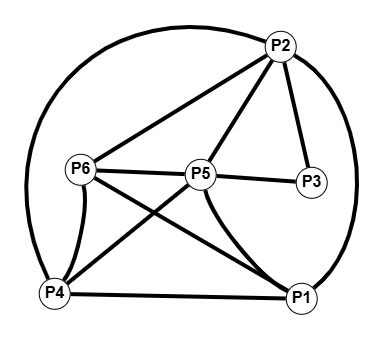
\includegraphics[width=0.7\textwidth, center]{attachments/9/1.png}
    \caption{Связи проектов}
    \label{fig:9_graph}
  \end{minipage}
\end{figure}
\begin{center}
Решение 
\end{center}
Построим граф $G$, представленный на рисунке \ref{fig:9_graph}, каждая вершина которого соответствует некоторому проекту, а ребро - наличию общих ресурсов, иначе говоря:
\begin{equation*}
(P_i,P_j) = 
 \begin{cases}
   1 &\text{$R_i \cap R_j \neq \varnothing$}\\
   0 &\text{иначе}
 \end{cases}
\end{equation*}
Проекты могут выполняться одновременно, если они не имеют общих ресурсов, то есть соответствующие проектам вершины не являются смежными. Соответственно, проекты $P_i$ и $P_j$ могут выполняться одновременно $\iff$ $P_i$ и $P_j$ принадлежат одному независимому множеству.\\
\\
Для выявления максимальных независимых множеств воспользуемся алгоритмом Брона-Кэрбоша:\\
\begin{enumerate}
    \item[\textit{Шаг 1}]$k = 0$
        \quad $S_0 = Q_0^{-} =\varnothing$,
        \quad  $Q_0^{+} = X = \{P_1,P_2,P_3,P_4,P_5,P_6\}$
    \item[\textit{Шаг 2}]
        $S_1 = \{P_5\}$,
        \quad  $Q_1^{+} =Q_0^{+} \hspace{1mm}\backslash\hspace{1mm} (\Gamma (P_5) \cup P_5) = \varnothing$,
        \quad  $Q_1^{-} = \varnothing$,
        \quad  $k = k + 1 = 1$
    \item[\textit{Шаг 3}] Условие не выполняется.
    \item[\textit{Шаг 4}] $Q_1^{-} = Q_1^{+} = \varnothing\quad\Longrightarrow \textbf{Максимальное Независимое Множество: }\{P_5\}$.
    \item[\textit{Шаг 5}] $k = k - 1 = 0$,
        \quad $S_0 =\varnothing$,
        \quad  $Q_0^{+} = \{P_1,P_2,P_3,P_4,P_6\}$,
        \quad  $Q_0^{-} = \{P_5\}$
    \item[\textit{Шаг 3}] Условие не выполняется.
    \item[\textit{Шаг 4}] $Q_0^{-} \neq \varnothing$,
        \quad $Q_0^{+}  \neq \varnothing$
    \item[\textit{Шаг 2}]
        $S_1 = \{P_1\}$,
        \quad  $Q_1^{+} = Q_0^{+} \hspace{1mm}\backslash\hspace{1mm} (\Gamma (P_1) \cup P_1) = \{P_3\}$,
        \quad  $Q_1^{-} = Q_0^{-} \hspace{1mm}\backslash\hspace{1mm} (\Gamma (P_1) \cup P_1) = \varnothing$,
        \quad  $k = k + 1 = 1$
    \item[\textit{Шаг 3}] Условие не выполняется.
    \item[\textit{Шаг 4}] $Q_1^{-} = \varnothing$,
    \quad$Q_1^{+} \neq \varnothing$
    \item[\textit{Шаг 2}]
        $S_2 = \{P_1, P_3\}$,
        \quad  $Q_2^{+} = Q_2^{+} \hspace{1mm}\backslash\hspace{1mm} (\Gamma (P_3) \cup P_3) = \varnothing$,
        \quad  $Q_2^{-} = \varnothing$,
        $k = k + 1 = 2$
    \item[\textit{Шаг 3}] Условие не выполняется.
    \item[\textit{Шаг 4}] $Q_2^{-} = Q_2^{+} = \varnothing\quad\Longrightarrow \textbf{Максимальное Независимое Множество: }\{P_1, P_3\}$.
    \item[\textit{Шаг 5}] $k = k - 1 = 1$,
        \quad $S_1 = \{P_1\}$,
        \quad $Q_1^{+} = \varnothing$,
        \quad  $Q_1^{-} = \{P_3\}$.
    \item[\textit{Шаг 3}] Условие не выполняется.
    \item[\textit{Шаг 4}] $Q_1^{+} = \varnothing$,
    \quad$Q_1^{-} \neq \varnothing$
    \item[\textit{Шаг 5}] $k = k - 1 = 0$,
        \quad $S_0 =\varnothing$,
        \quad  $Q_0^{+} = \{P_3,P_2,P_4,P_6\}$,
        \quad  $Q_0^{-} = \{P_5,P_1\}$
    \item[\textit{Шаг 3}]  Условие не выполняется.
    \item[\textit{Шаг 4}] $Q_0^{+} \neq \varnothing$,
    \quad$Q_0^{-} \neq \varnothing$
    \item[\textit{Шаг 2}]
        $S_1 = \{P_2\}$,
        \quad  $Q_1^{+} = Q_0^{+} \hspace{1mm}\backslash\hspace{1mm} (\Gamma (P_2) \cup P_2) = \varnothing$,
        \quad  $Q_1^{-} = \varnothing$,
        \quad  $k = k + 1 = 1$
    \item[\textit{Шаг 3}] Условие не выполняется.
    \item[\textit{Шаг 4}] $Q_1^{-} = Q_1^{+} = \varnothing\quad\Longrightarrow \textbf{Максимальное Независимое Множество: }\{P_2\}$.
    \item[\textit{Шаг 5}] $k = k - 1 = 0$,
        \quad $S_0 = \varnothing$,
        \quad $Q_0^{+} = \{P_3,P_4,P_6\}$,
        \quad  $Q_0^{-} = \{P_1,P_2,P_5\}$.
    \item[\textit{Шаг 3}]  Условие не выполняется.
    \item[\textit{Шаг 4}] $Q_0^{+} \neq \varnothing$,
    \quad$Q_0^{-} \neq \varnothing$
    \item[\textit{Шаг 2}]
        $S_1 = \{P_4\}$,
        \quad  $Q_1^{+} = Q_0^{+} \hspace{1mm}\backslash\hspace{1mm} (\Gamma (P_4) \cup P_4) = = \{P_3\}$,
        \quad  $Q_1^{-} = Q_0^{-} \hspace{1mm}\backslash\hspace{1mm} (\Gamma (P_4) \cup P_4) = \varnothing$,
        \quad  $k = k + 1 = 1$
    \item[\textit{Шаг 3}] Условие не выполняется.
    \item[\textit{Шаг 4}] $Q_1^{-} = \varnothing$,
    \quad$Q_1^{+} \neq \varnothing$
    \item[\textit{Шаг 2}]
        $S_2 = \{P_4, P_3\}$,
        \quad  $Q_2^{+} = Q_2^{+} \hspace{1mm}\backslash\hspace{1mm} (\Gamma (P_3) \cup P_3) = \varnothing$,
        \quad  $Q_2^{-} = \varnothing$,
        \quad  $k = k + 1 = 2$
    \item[\textit{Шаг 3}] Условие не выполняется.
    \item[\textit{Шаг 4}] $Q_2^{-} = Q_2^{+} = \varnothing\quad\Longrightarrow \textbf{Максимальное Независимое Множество: }\{P_4, P_3\}$.
    \item[\textit{Шаг 5}] $k = k - 1 = 1$,
        \quad $S_1 = \{P_4\}$,
        \quad $Q_1^{+} = \varnothing$,
        \quad  $Q_1^{-} = \{P_3\}$.
    \item[\textit{Шаг 3}] Условие не выполняется.
    \item[\textit{Шаг 4}] $Q_1^{+} = \varnothing$,
    \quad$Q_1^{-} \neq \varnothing$
    \item[\textit{Шаг 5}] $k = k - 1 = 0$,
        \quad $S_0 =\varnothing$,
        \quad  $Q_0^{+} = \{P_3,P_6\}$,
        \quad  $Q_0^{-} = \{P_5,P_1,P_2,P_4\}$
    \item[\textit{Шаг 3}]  Условие не выполняется.
    \item[\textit{Шаг 4}] $Q_0^{+} \neq \varnothing$,
    \quad$Q_0^{-} \neq \varnothing$
    \item[\textit{Шаг 2}]
        $S_1 = \{P_6\}$,
        \quad  $Q_1^{+} = Q_0^{+} \hspace{1mm}\backslash\hspace{1mm} (\Gamma (P_6) \cup P_6) = \{P_3\}$,
        \quad  $Q_1^{-} = Q_0^{-} \hspace{1mm}\backslash\hspace{1mm} (\Gamma (P_6) \cup P_6) = \varnothing$,
        \quad  $k = k + 1 = 1$
    \item[\textit{Шаг 3}] Условие не выполняется.
    \item[\textit{Шаг 4}] $Q_1^{-} = \varnothing$,
    \quad$Q_1^{+} \neq \varnothing$
    \item[\textit{Шаг 2}]
        $S_2 = \{P_6, P_3\}$,
        \quad  $Q_2^{+} = Q_2^{+} \hspace{1mm}\backslash\hspace{1mm} (\Gamma (P_3) \cup P_3) = \varnothing$,
        \quad  $Q_2^{-} = \varnothing$,
        \quad  $k = k + 1 = 2$
    \item[\textit{Шаг 3}] Условие не выполняется.
    \item[\textit{Шаг 4}] $Q_2^{-} = Q_2^{+} = \varnothing\quad\Longrightarrow \textbf{Максимальное Независимое Множество: }\{P_6, P_3\}$. 
    \item[\textit{Шаг 5}] $k = k - 1 = 1$,
        \quad $S_1 = \{P_6\}$,
        \quad $Q_1^{+} = \varnothing$,
        \quad  $Q_1^{-} = \{P_3\}$.
    \item[\textit{Шаг 3}] Условие не выполняется.
    \item[\textit{Шаг 4}] $Q_1^{+} = \varnothing$,
    \quad$Q_1^{-} \neq \varnothing$
    \item[\textit{Шаг 5}] $k = k - 1 = 0$,
        \quad $S_0 =\varnothing$,
        \quad  $Q_0^{+} = \{P_3\}$,
        \quad  $Q_0^{-} = \{P_5,P_1,P_2,P_4,P_6\}$
    \item[\textit{Шаг 3}] Условие выполняется: $\exists x_1 \in Q_0^{-}: \Gamma (x_1) \cap Q_0^{+} = \varnothing$
    \item[\textit{Шаг 5}] $k = 0$,
        \quad $S_0 =\varnothing$,
        \quad  $Q_0^{+} = \varnothing$,
        \quad  $Q_0^{-} = \{P_1,P_2,P_3,P_4,P_5,P_6\}$\\
        $k = 0, \quad Q_0^{+} =\varnothing\quad\Longrightarrow \text{\textbf{Критерий останова:} перечислены все максимальные независимые множества.}$
    \\
    \\
\end{enumerate}
% \begin{figure}[h]
%     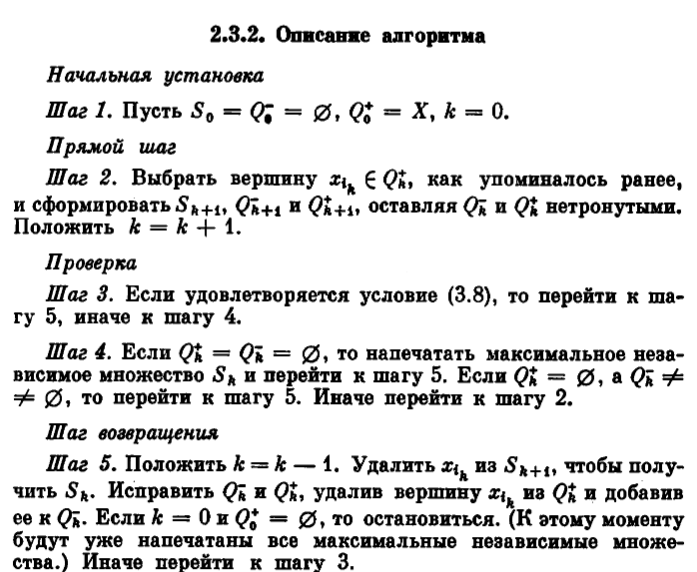
\includegraphics[width=0.6\textwidth, center]{attachments/4/algo.png}
%     \caption{Алгоритм}
%     \label{fig:figure4_algo}
% \end{figure}
Таким образом, исходя из полученных максимальных независимых множеств ввиду совместного пользования ресурсами одновременно могут выполняться:
\begin{enumerate}
    \item[либо] $P_5$, 
    \item[либо] $P_2$,
    \item[либо] $P_1$ и $P_3$,
    \item[либо] $P_4$ и $P_3$,
    \item[либо] $P_6$ и $P_3$.
\end{enumerate}
\end{enumerate}


\clearpage% 10------------------------------------------
\begin{enumerate}
\item[\textbf{Задача 10.}] Предположим, что вычислительная система включает $n$ вычислительных устройств разной производительности для решения $n$ типов задач. Временные затраты на решение задачи $i$-го типа $j$-ым устройством заданы в форме матрицы $C$, представленной на таблице \ref{tab:10_Cmatrix}. Определить такое распределение задач между вычислительными устройствами, чтобы затраты времени на обработку пакета из $n$ различных задач были минимальными.
\begin{table}[!ht]
    \centering
    \begin{tabular}{|c|c|c|c|c|c|c|}
    \hline
        & \textit{A} & \textit{B} & \textit{C} & \textit{D} & \textit{E} & \textit{F} \\ \hline
        \textit{a} & 2 & 3 & 5 & 5 & 8 & 1 \\ \hline
        \textit{b} & 13 & 4 & 7 & 6 & 4 & 10 \\ \hline
        \textit{c} & 7 & 18 & 3 & 4 & 2 & 6 \\ \hline
        \textit{d} & 5 & 9 & 7 & 8 & 4 & 9 \\ \hline
        \textit{e} & 10 & 12 & 8 & 17 & 9 & 11 \\ \hline
        \textit{f} & 3 & 4 & 5 & 7 & 8 & 4 \\ \hline
    \end{tabular}
    \caption{Матрица временных затрат}
    \label{tab:10_Cmatrix}
\end{table}
\begin{center}
Решение 
\end{center}
\begin{figure}[ht]
     \centering
     \begin{subfigure}[b]{0.3\textwidth}
        \centering
         \caption*{\small{Приведем стоимостную матрицу $C$ по строкам: вычтем из каждого элемента $min$ по строке}}
         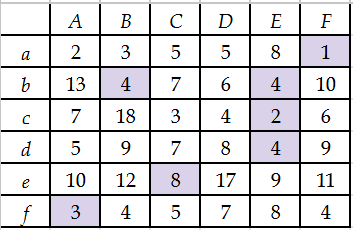
\includegraphics[width=\textwidth]{attachments/10/01.png}
         \label{fig:10_01}
     \end{subfigure}
     \hfill
     \begin{subfigure}[b]{0.3\textwidth}
        \centering
         \caption*{\small{Приведем получившуюся матрицу $C$ по столбцам: вычтем из каждого элемента $min$ по столбцу}}
         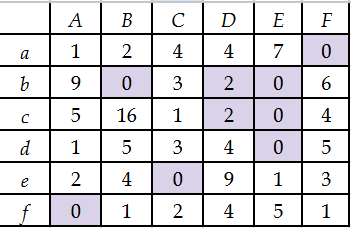
\includegraphics[width=\textwidth]{attachments/10/02.png}
         \label{fig:10_02}
     \end{subfigure}
     \hfill
     \begin{subfigure}[b]{0.3\textwidth}
         \centering
         \caption*{\small{Приведенная матрица}}
         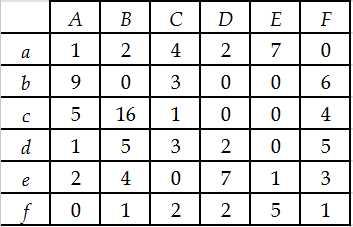
\includegraphics[width=\textwidth]{attachments/10/03.png}
         \label{fig:10_03}
        \end{subfigure}
    \hfill
     \begin{subfigure}[b]{0.3\textwidth}
         \centering
         \caption*{\small{$k = 6 = n$; соответственно, решение задачи получено}}
         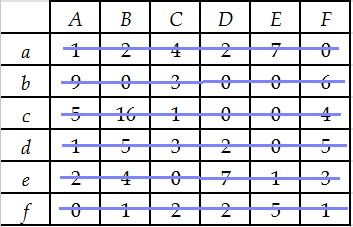
\includegraphics[width=\textwidth]{attachments/10/031.png}
         \label{fig:10_031}
     \end{subfigure}
     \hfill
     \begin{subfigure}[b]{0.3\textwidth}
         \centering
         \caption*{\small{Выделим независимые нули, полученные в результате алгоритма поиска максимальных паросочетаний, произведенного на рисунке \ref{fig:10_max_pairs}}}
         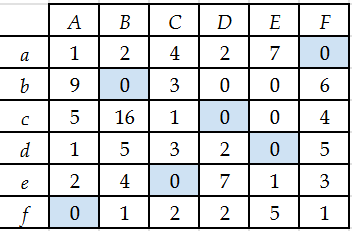
\includegraphics[width=\textwidth]{attachments/10/04.png}
         \label{fig:10_04}
     \end{subfigure}
     \hfill
     \begin{subfigure}[b]{0.3\textwidth}
         \centering
         \caption*{\small{В исходной матрице выделенным нулям соответствует сумма временных затрат $\sum = 24$}}
         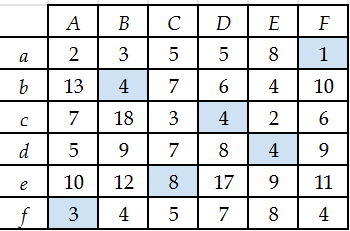
\includegraphics[width=\textwidth]{attachments/10/05.png}
         \label{fig:10_05}
     \end{subfigure}
    \caption{Преобразования стоимостной матрицы}
    \label{fig:10_matrix_changes}
\end{figure}
\begin{figure}
     \centering
     \begin{subfigure}[t]{0.32\textwidth}
        \centering
         \caption*{\small{Преобразуем граф: ориентируем, добавим сток и источник}}
         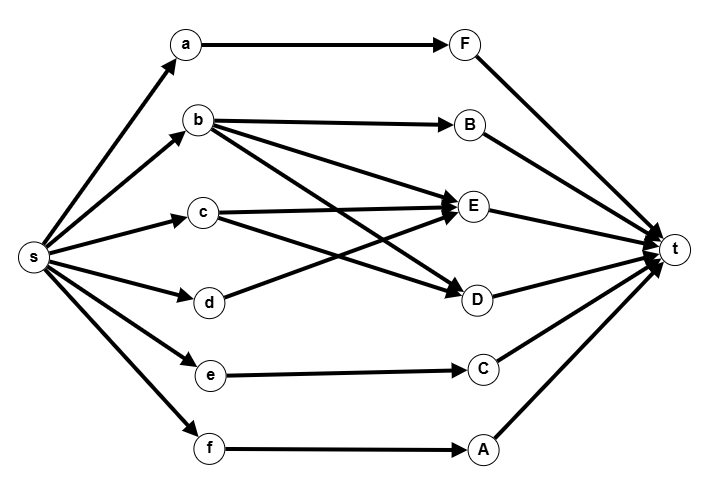
\includegraphics[width=\textwidth]{attachments/10/0.png}
         \label{fig:10_0}
     \end{subfigure}
     \hfill
     \begin{subfigure}[t]{0.32\textwidth}
        \centering
         \caption*{\small{$\mu_1 = [s, a, F, t]$\\$P =\{(a,F)\}$}}
        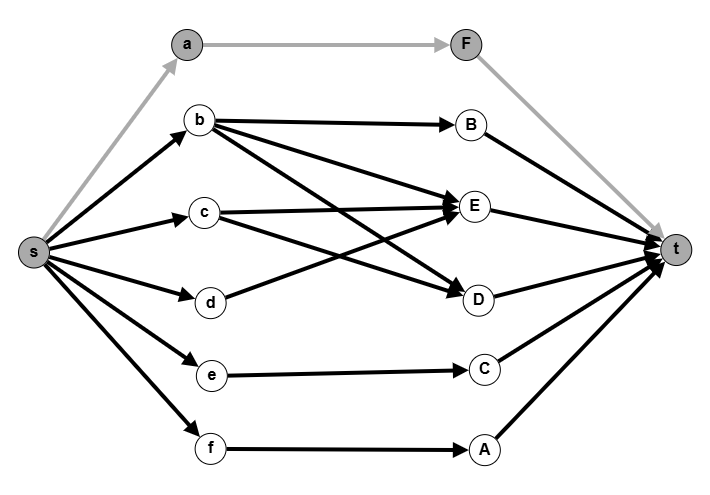
\includegraphics[width=\textwidth]{attachments/10/1.png}
         \label{fig:10_1}
     \end{subfigure}
     \hfill
     \begin{subfigure}[t]{0.32\textwidth}
        \centering
         \caption*{\small{$\mu_2 = [s, f, A, t]$\\$P =\{(a,F),(f,A)\}$}}
         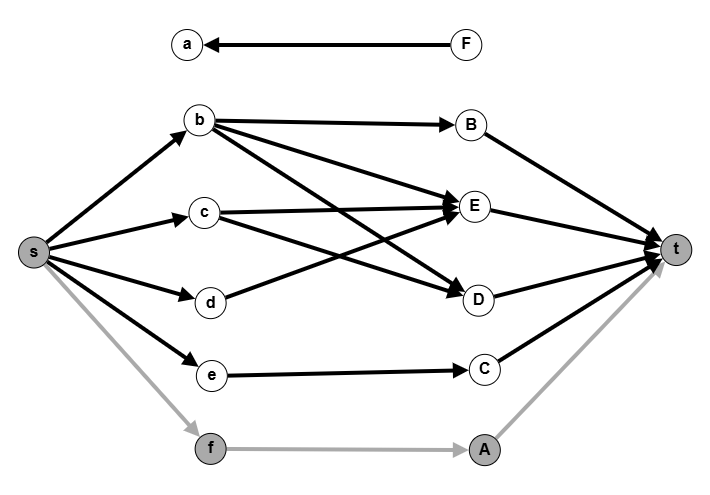
\includegraphics[width=\textwidth]{attachments/10/2.png}
         \label{fig:10_2}
     \end{subfigure}
     \hfill
     \begin{subfigure}[t]{0.32\textwidth}
        \centering
         \caption*{\small{$\mu_3 = [s, e, C, t]$\\$P =\{(a,F),(f,A),(e, C)\}$}}
         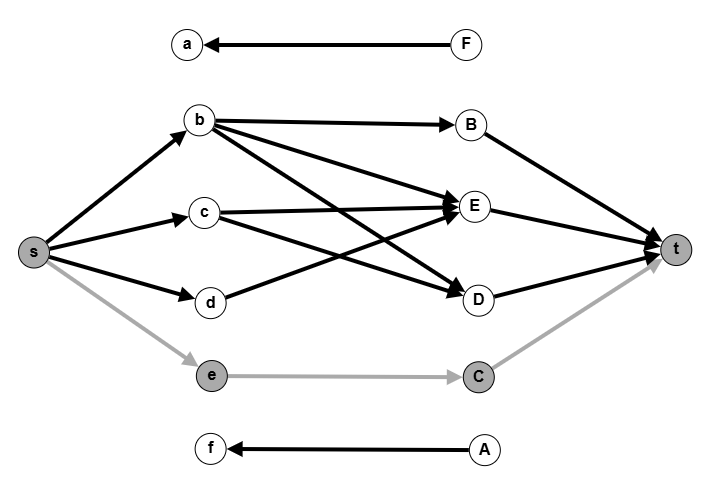
\includegraphics[width=\textwidth]{attachments/10/3.png}
         \label{fig:10_3}
     \end{subfigure}
      \hfill
     \begin{subfigure}[t]{0.32\textwidth}
        \centering
         \caption*{\small{$\mu_4 = [s, b, D, t]$\\$P =\{(a,F),(f,A),(e, C), (b, D)\}$}}
         \includegraphics[width=\textwidth]{attachments/10/4.png}
         \label{fig:10_4}
     \end{subfigure}
    \hfill
     \begin{subfigure}[t]{0.32\textwidth}
        \centering
         \caption*{\small{$\mu_5 = [s, c, D, b, B, t]$\\$P =\{(a,F),(f,A),(e, C), (c,D), (b,B)\}$}}
         \includegraphics[width=\textwidth]{attachments/10/5.png}
         \label{fig:10_5}
     \end{subfigure}
    \hfill
     \begin{subfigure}[t]{0.32\textwidth}
        \centering
         \caption*{\small{$\mu_6 = [s, d,E,t]$\\$P =\{(a,F),(f,A),(e, C), (c,D), (b,B), (d, E)\}$}}
         \includegraphics[width=\textwidth]{attachments/10/6.png}
         \label{fig:10_6}
     \end{subfigure}
     \hfill
     \begin{subfigure}[t]{0.32\textwidth}
        \centering
         \caption*{\small{$P =\{(a,F),(f,A),(e, C), (c,D), (b,B), (d, E)\}$}}
         \includegraphics[width=\textwidth]{attachments/10/7_.png}
         \label{fig:10_7}
     \end{subfigure}
    \caption{Процесс построения максимального паросочетания}
    \label{fig:10_max_pairs}
\end{figure}
Как отражено на рисунке \ref{fig:10_matrix_changes}, минимальные затраты времени на обработку пакета из $n = 6$ различных задач при заданной таблицей \ref{tab:10_Cmatrix} матрице затрат времени $C$ составляют 24 и соответствующее распределение задач между вычислительными устройствами представлено в таблице \ref{tab:10_res}.
% \begin{tabular}         
%     {|l|c|c|c|c|c|c|}
%     \hline
%         \textit{№ вычислительной задачи} & 1 & 2 & 3 & 4 & 5 & 6 \\ \hline
%         \textit{№ устройства} & 6 & 2 & 4 & 5 & 3 & 1 \\ \hline
% \end{tabular}
\begin{table}
    \centering
    \begin{tabular}{c|c}
        \textit{№ задачи} & \textit{№ устройства} \\ \hline
        1 & 6 \\
        2 & 2 \\
        3 & 4 \\
        4 & 5 \\
        5 & 3 \\
        6 & 1 \\ \hline
    \end{tabular}
    \caption{Соответствие вычислительной задачи и выполняющего ее устройства}
    \label{tab:10_res}
\end{table}
\end{enumerate}


\clearpage% 11------------------------------------------
\begin{enumerate}
\item[\textbf{Задача 11.}]Для «задачи о свадьбах» четко сформулируйте алгоритм, придумайте иллюстративный пример для двудольного графа $K_{5,5}$, изображенного на рисунке \ref{fig:11_graph}. Подробно распишите шаги алгоритма.\\
\begin{center}
Решение 
\end{center}
Пусть $X$\quad\textendash\quad множество юношей, $Y$\quad\textendash\quad  множество девушек, а наличие ребра $(x,y)$ означает, что $x$ и $y$
могут поженится, тогда паросочетание есть коллективная свадьба, в которой каждый заключает не более одного брака. 
Ясно, что в реальной жизни лицо имеет предпочтения, и эту особенность необходимо учитывать в нашей ситуации. Предположим, что для каждой 
вершины $v \in X \cup Y$ задано упорядочение вершин 
$R(v) = \left\{z_1 \succ z_2 \succ \cdots \succ z_{d(v)} \right\} $, 
которые с ней смежны, при этом на первом месте стоит вершина
$z_1$, которой соответствует наиболее предпочтительное лицо, а на последнем месте\quad\textendash\quad$z_{d(v)}$\quad\textendash\quad наименее предпочтительное лицо.\\
Паросочетание $P$ в двудольном графе $G = (X \cup Y, E)$
называется устойчивым, если для любого ребра $(u,v)\in E\backslash P$, где $u \in X$, $v \in Y$,

\qquad\qquadлибо $(u,y) \in P$ и $y \succ v$  в $R(u)$,

\qquad\qquadлибо $(x,v) \in P$ и $x \succ u$  в $R(v)$,

\qquad\qquadлибо выполняется и то, и другое.\\
В нашей интерпретации множество бракосочетаний устойчиво, если в нем отсутствуют ситуации, когда брак между $u \in R(v)$ и $v \in R(u)$
не заключен, но $u$ предпочитает $v$ своей жене (или не женат), а 
$v$ предпочитает $u$ своему мужу (или не замужем).\\
\\
Алгоритм следующий: на первом шаге все юноши
$u \in X$ делают предложения своим самым желанным девушкам. Если девушка получает хотя бы одно предложение, она выбирает наиболее желанного юношу и считает его кандидатом в женихи. Оставшиеся юноши отвергнуты и образуют резерв $T$, все юноши из которого на втором шаге
делают предложения своим вторым по предпочтениям девушкам. Каждая девушка сравнивает предложения, учитывая кандидата в женихи, если таковой имеется, выбирает наиболее предпочтительного юношу и делает его кандидатом в женихи. Отвергнутые юноши составляют новый резерв $T$.
После этого юноши из $T$ делают предложения своим следующим по предпочтениям девушкам, и так далее.
Юноша, который сделал предложение последней по его предпочтениям девушке и был отвергнут, исключается из
дальнейшего рассмотрения, а также из резерва. Очевидно, что через некоторое время резерв $T$ окажется пустым, и в этот момент алгоритм заканчивает работу.
\begin{enumerate}
    \item[\textbf{S1}] Формируются пары $(u_i,v)$  $\forall u_i \in X$, где $v = z_\text{наиб предпочтительное из еще не использованных} \in R(u_i)$, $v \in Y$. В строящееся паросочетание отбираются пары $(u_i^*, v)$ такие, что $u_i^* = z_{\text{наиб предпочтительное из }u \in\Gamma(v)} \in R(v)$\\
    Множество резерва формируется как множество $T = \{u\in X: (u,v) \not\in P, v \in Y\}$. 

    \item[\textbf{S2}] Пока $T \neq \varnothing$ повторять:
    
    Формируются пары $(u_t,v)$  $\forall u_t \in T$, где $v = z_\text{наиб предпочтительное из еще не использованных} \in R(u_i)$, $v \in Y$. Строящееся паросочетание обновляется для всех $v$:\\
    если $(u, v) \not\in P, \forall u \in X$, то $P = P \cup (u_t, v)$;\\
    
    если $(u, v) \in P, u \in X$
    
    \qquad\qquad и $u_t \succ u$, то $P = (P\backslash(u, v)) \cup (u_t, v)$, $T = (T\backslash \{u_t\}) \cup {u}$

    \qquad\qquad иначе если $v = z_5 \in R(u_t)$, то $T = T\backslash \{u_t\}$ и $u_t$ исключается из дальнейшего рассмотрения.

    
    такие, что $u_i^* = z_{\text{наиб предпочтительное из }u \in\Gamma(v_j)} \in R(v_j)$\\
    Множество резерва формируется как множество $T = \{u\in X: u \not\in P\}$.
\end{enumerate}
\begin{figure}[ht]
    \includegraphics[width=0.7\textwidth, center]{attachments/11/full/0.png}
    \caption{Двудольный граф $K_{5,5}$}
    \label{fig:11_graph}
\end{figure}
Проиллюстрируем работу алгоритма на примере. Рассмотрим граф $K_{5,5}$, изображенный на рисунке \ref{fig:11_graph}.
\begin{enumerate}
    \item[\textit{Шаг 1}] Юноши делают предложения, исходя из высшей предпочтительности:\qquad $(a,A),(b,A),(c,C),(d,C),(e,A)$\\
    Девушки, выбирая наиболее предпочтительный вариант из предложенных, формируют кандидатов в женихи:\qquad $(e,A),(c,C)$\\
    Резерв на шаге:\qquad $T =\{a,b,d\}$ 
    
    \item[\textit{Шаг 2}] Юноши, находящиеся в резерве, делают предложения своим вторым по предпочтениям девушкам:\qquad $(a,C),(b,E),(d,E)$\\
    Девушки, выбирая наиболее предпочтительный вариант из предложенных, дополняют список кандидатов в женихи:\qquad $(e,A),(c,C),(d,E)$\\
    Резерв на шаге:\qquad $T =\{a,b\}$
    
    \item[\textit{Шаг 3}] Юноши, находящиеся в резерве, делают предложения своим третьим по предпочтениям девушкам:\qquad $(a,B),(b,B)$\\
    Девушки, выбирая наиболее предпочтительный вариант из предложенных, дополняют список кандидатов в женихи:\qquad $(e,A),(b,B),(c,C),(d,E)$\\
    Резерв на шаге:\qquad $T =\{a\}$
    
    \item[\textit{Шаг 4}] Юноша $a$, единственный находящийся в резерве, делает предложения своим четвертым по предпочтениям девушкам:\qquad $(a,E)$\\
    Девушка $E$, выбирая наиболее предпочтительный вариант из предложенных \quad\textemdash\quad $a \succ d$, изменяют список кандидатов в женихи:\qquad $(e,A),(b,B),(c,C),(a,E)$\\
    Резерв на шаге:\qquad $T =\{d\}$
    
    \item[\textit{Шаг 5}] Юноша $d$, единственный находящийся в резерве, делает предложения своей третьей по предпочтениям девушке:\qquad $(d,A)$\\
    Девушка $A$, выбирая наиболее предпочтительный вариант из предложенных \quad\textemdash\quad $e \succ d$, отклоняет предложение, и список остается без изменений:\qquad  $(e,A),(b,B),(c,C),(a,E)$\\
    Резерв на шаге:\qquad $T =\{d\}$
    
    \item[\textit{Шаг 6}] Юноша $d$, единственный находящийся в резерве, делает предложения своей четвертой по предпочтениям девушке:\qquad $(d,B)$\\
    Девушка $B$, выбирая наиболее предпочтительный вариант из предложенных \quad\textemdash\quad $d \succ b$, принимает предложение, видоизменяя список кандидатов:\qquad $(e,A),(d,B),(c,C),(a,E)$\\
    Резерв на шаге:\qquad $T =\{b\}$

    \item[\textit{Шаг 7}] Юноша $b$, единственный находящийся в резерве, делает предложения своей четвертой по предпочтениям девушке:\qquad $(b,D)$\\
    Девушке $D$ до этого поступало предложений и в силу отсутствия иных вариантов, предложение принимается, дополняя список кандидатов:\qquad $(e,A),(d,B),(c,C),(b,D),(a,E)$\\
    Резерв на шаге:\qquad $T =\{\varnothing\}$   
\end{enumerate}
Резерв $T =\{\varnothing\} \Longrightarrow$ \textbf{критерий останова}. Таким образом, в результате применения алгоритма было получено устойчивое паросочетание $P = \{(e,A),(d,B),(c,C),(b,D),(a,E)\}$.
\clearpage
\begin{center}
Пример для изображенного на рисунке \ref{fig:to_bin_11_graph} неполного двудольного графа, выполненный по невнимательности при прочтении условия, однако все еще иллюстрирующий работу алгоритма, хотя и не так наглядно, как описанный выше пример для полного графа.
\end{center}
\begin{figure}[ht]
    \includegraphics[width=0.7\textwidth, center]{attachments/11/00.png}
    \caption{Неполный двудольный граф $G_{5,5}$}
    \label{fig:to_bin_11_graph}
\end{figure}
\begin{figure}
     \centering
     \begin{subfigure}[b]{0.47\textwidth}
        \centering
         \caption*{Формируются предложения:\\ $a\rightarrow D,\quad b\rightarrow A,\quad c\rightarrow B,\quad d\rightarrow E,\quad e\rightarrow D$ \\
         Исходя из предпочтительности, кандидаты:\\ 
         $b\rightarrow A,\quad c\rightarrow B,\quad d\rightarrow E,\quad e\rightarrow D$ \\
         Резерв на шаге:
         $T =\{a\}$}
         \includegraphics[width=\textwidth]{attachments/11/11.png}
         \label{fig:to_bin_11_1}
     \end{subfigure}
     \hfill
          \begin{subfigure}[b]{0.47\textwidth}
        \centering
         \caption*{Формируются предложения: $a\rightarrow B$ \\
         Исходя из предпочтительности, так как для $B$ $c \succ a$, предложение отвергается.\\
         Резерв на шаге:
         $T =\{a\}$}
         \includegraphics[width=\textwidth]{attachments/11/22.png}
         \label{fig:to_bin_11_2}
     \end{subfigure}
          \hfill
    \begin{subfigure}[b]{0.47\textwidth}
        \centering
         \caption*{Формируются предложения: $a\rightarrow C$
         \\Исходя из того, что для $C$ не было других предложений, предложение принимается.\\
         Резерв на шаге: $T =\{\varnothing\}$}
         \includegraphics[width=\textwidth]{attachments/11/33.png}
         \label{fig:to_bin_11_3}
     \end{subfigure}
     \hfill
     \begin{subfigure}[b]{0.47\textwidth}
        \centering
         \caption*{Резерв $T =\{\varnothing\}$ - \textbf{критерий останова}.\\
         Сформированное устойчивое сочетание:\\
         $P = \{(a,C),(b,A),(c,B),(d,E),(e,D)\}$
         }
         \includegraphics[width=\textwidth]{attachments/11/44.png}
         \label{fig:to_bin_11_4}
     \end{subfigure}
     \caption{Этапы решения задачи}
    \label{fig:to_bin_11_max_pairs}
\end{figure}
\clearpage

\end{enumerate}


\clearpage% 12-----------------------------------
\begin{enumerate}
\item[\textbf{Задача 12.}]В период прохождения обучения в летней IT-школе, организованной компанией «PaRus», за каждым слушателем закрепляется наставник. В результате собеседования каждый из трех обучающихся указал наиболее предпочтительные кандидатуры наставников. На рисунке \ref{fig:12_initree} представлен граф, который отражает эти предпочтения. Каждое ребро определяет назначение слушателю одного из наставников, но у каждого слушателя должен быть только один наставник. Укажите наставника для каждого слушателя с учетом его предпочтений.
\begin{figure}[ht]
    \includegraphics[width=0.27\textwidth, center]{attachments/12/12_graph.png}
    \caption{Предпочтения слушателей к наставникам}
    \label{fig:12_initree}
\end{figure}
% \begin{figure}[ht]
%   \begin{minipage}[b]{0.5\textwidth}
%     \centering
%     \includegraphics[width=0.5\textwidth, center]
%     {attachments/12/12_graph.png}
%     \caption{Предпочтения слушателей к наставникам}
%     \label{fig:12_initree}
%   \end{minipage}
%   \hfill
%   \begin{minipage}[b]{0.5\textwidth}
%     \centering
%     \includegraphics[width=0.5\textwidth, center]
%     {attachments/12/12_pairs.png}
%     \caption{Сформированные пары слушатель-наставник}
%     \label{fig:12_res_pairs}
%   \end{minipage}
% \end{figure}
\begin{center}
Решение 
\end{center}
Для выявления наставника для каждого слушателя с учетом его предпочтений используем алгоритм построения максимального паросочетания в двудольном графе, изображенный поэтапно на рисунке \ref{fig:12_max_pairs}. Заметим, что, в силу нечетности числа вершин графа, совершенного паросочетания не существует, то есть - в контексте задачи - у одного из наставников не будет слушателя.
\\
\\
Таким образом, сформированные пары из слушателя и наставника представлены на рисунке \ref{fig:12_res_pairs}.
\begin{figure}[ht]
    \includegraphics[width=0.27\textwidth, center]{attachments/12/12_pairs.png}
    \caption{Сформированные пары слушатель-наставник}
    \label{fig:12_res_pairs}
\end{figure}
\begin{figure}
     \centering
     \begin{subfigure}[b]{0.35\textwidth}
        \centering
         \caption*{Преобразуем граф:добавим вершины стока s и источника t,  ориентируем ребра по направлению из s в t:}
         \includegraphics[width=\textwidth]{attachments/12/0.png}
         \label{fig:12_0}
     \end{subfigure}
     \hfill
     \begin{subfigure}[b]{0.35\textwidth}
        \centering
         \caption*{$\mu_1 = [s, C1, H4, t]$\\$P =\{(C1, H4)\}$}
        \includegraphics[width=\textwidth]{attachments/12/1.png}
         \label{fig:12_1}
     \end{subfigure}
     \hfill
     \begin{subfigure}[b]{0.35\textwidth}
        \centering
         \caption*{$\mu_2 = [s, C3, H1, t]$\\$P =\{(C1, H4), (C3, H1)\}$}
        \includegraphics[width=\textwidth]{attachments/12/2.png}
         \label{fig:12_2}
     \end{subfigure}
     \hfill
     \begin{subfigure}[b]{0.35\textwidth}
        \centering
         \caption*{$\mu_3 = [s, C2, H4, C1, H1, C3, H3, t]$\\$P =\{(C2, H4),(C1, H1), (C3, H3)\}$}
        \includegraphics[width=\textwidth]{attachments/12/3.png}
         \label{fig:12_3}
     \end{subfigure}
     \hfill
     \begin{subfigure}[b]{0.37\textwidth}
        \centering
         \caption*{Критерий останова: нет более доступных путей из источника.}
        \includegraphics[width=\textwidth]{attachments/12/4.png}
         \label{fig:12_4}
     \end{subfigure}
     \caption{Процесс построения максимального паросочетания}
    \label{fig:12_max_pairs}
\end{figure}
\end{enumerate}


\clearpage% 13------------------------------------------
\begin{enumerate}
\item[\textbf{Задача 13.}] Найти максимальное паросочетание в чередующемся дереве, представленном на рисунке \ref{fig:13_initree}.
\begin{figure}[ht]
    \includegraphics[width=0.3\textwidth, center]{attachments/13/00.png}
    \caption{Чередующееся дерево}
    \label{fig:13_initree}
\end{figure}
\begin{center}
Решение 
\end{center}
Чередующееся дерево \quad\textemdash\quad дерево, вершины которого разбиты на два подмножества \quad\textemdash\quad внутренние и внешние \quad\textemdash\quad при этом каждое ребро соединяет внутреннюю вершину с внешней и степень каждой из внутренних вершин составляет 2.

\begin{figure}[!htp]
\begin{subfigure}{\textwidth}
\caption*{\textbf{S1.}Получим разбиение вершин на внутренние, выделенные цветом, и внешние:}
\centering
\includegraphics[width=0.49\textwidth]{attachments/13/1.png}
\end{subfigure}
\vspace{10px}
\begin{subfigure}{\textwidth}
\centering
\caption*{\textbf{S2.} Выберем в качестве ведущей вершины $x_0$ произвольную вершину из множества внешних вершин
$x_0 = c$ и положим ей в соот-вие метку $d_0 = 0$.
В качестве меток для остальных вершин примем длину кратчайшей цепи от данной вершины к вершине $x_0$. Получим:}
\includegraphics[width=0.49\textwidth]{attachments/13/2.png}
\end{subfigure}
\vspace{10px}
\begin{subfigure}{\textwidth}
\centering
\caption*{\textbf{S3.} В максимальное паросочетание включим такие ребра $( x_i^{внутр}, x_j^{внешн})$, 
для концевых вершин которых будет верно: $d_j = d_i + 1$}
\includegraphics[width=0.49\textwidth]{attachments/13/3_coloured.png}
\end{subfigure}
\vspace{10px}
\begin{subfigure}{\textwidth}
\caption*{\textbf{S4.} Таким образом, максимальное паросочетание данного графа включает в себя следующие ребра:}
\centering
\includegraphics[width=0.49\textwidth]{attachments/13/3.png}
\end{subfigure}
% \bigskip
% \begin{subfigure}{\textwidth}
% \includegraphics[width=\textwidth,height=8cm]{attachments/13/3.png}
% \caption*{\textbf{S4.} Таким образом, максимальное паросочетание данного графа включает в себя следующие ребра:}
% \end{subfigure}
\caption{Нахождения максимального паросочетания в чередующемся дереве}
\label{fig:13_steptrees}
\end{figure}

\end{enumerate}


\clearpage% 14------------------------------------------
\begin{enumerate}
\item[\textbf{Задача 14.}]Модифицировать алгоритм Прима для нахождения остова максимального суммарного веса и привести иллюстративный пример.
\\
\begin{center}
Решение 
\end{center}
Для нахождения остова максимального суммарного веса модифицируем алгоритм Прима следующим образом:
\begin{enumerate}
    \item начальные метки имеют значение
    \item на каждой итерации выбирается
\end{enumerate}
При помощи модифицированного алгоритма построим остов максимального веса для графа, изображенного на рисунке \ref{fig:14_graph}. Итерации отражены в таблице на рисунке \ref{fig:14_matrix}, при этом цветом выделена метка, выбранной на данном шаге вершины, и жирным шрифтом выделены метки смежных ей вершин.  
\begin{figure}[ht]
    \centering
    \includegraphics[width=0.6\textwidth, center]{attachments/8/0.png}
    \caption{Граф}
    \label{fig:14_graph}
\end{figure}
\begin{figure}[ht]
    \centering
    \includegraphics[width=\textwidth, center]{attachments/14/matrix.png}
    \caption{Таблица итераций алгоритма}
    \label{fig:14_matrix}
\end{figure}
\\
Таким образом, вес найденного остова максимального суммарного веса составляет:
$$7+14+13+9+8+10+10+10+9+8+7 = 105$$
% представлен на рисунке \ref{fig:14_ostov} и его вес 
\end{enumerate}


\clearpage% 15------------------------------------
\begin{enumerate}
\item[\textbf{Задача 15.}] Тематика предстоящей летней школы включает разделы передовых технологий программирования. Всего предполагается прочитать 10 лекций, причем в определенной последовательности Л1-Л10. С учетом занятости сотрудников, читающих лекции, предполагается следующее распределение: Иванов А.А. – Л1, Л4, Л6, Л10; Сергеев А.Д. – Л2, Л3, Л7, Л9; Петров В.С. – Л5, Л8. Предполагается, что продолжительность лекции составляет 1.5 часа, и в день планируется не более трех лекций. Для составления расписания предложено построить математическую модель в виде неориентированного графа, в котором вершины соответствуют лекциям, и две вершины соединяются ребром, когда они не могут быть прочитаны одновременно (например, их должен читать один и тот же сотрудник, возможны и другие причины). Соответствующий граф представлен на рисунке \ref{fig:15_graph}. Предложите такое расписание для чтения лекций, чтобы был соблюден их порядок, и на это было затрачено минимальное количество часов. 
\begin{figure}[ht]
    \includegraphics[width=0.3\textwidth, center]{attachments/15/15_0.png}
    \caption{Граф связи между лекциями}
    \label{fig:15_graph}
\end{figure}
\begin{center}
Решение 
\end{center}
Для выделения расписания, приняв номер предполагаемого дня проведения лекции за номер цвета, воспользуемся следующей процедурой раскраски графа: в один цвет окрашивается некоторое максимальное независимое множество, затем окрашенные вершины вместе с инцидентными ребрами удаляются из графа и в следующий цвет окрашивается некоторое максимальное независимое множество обновленного графа, при этом шаги процедура повторяется до тех пор пока не будут раскрашены все вершины. Итерации алгоритма представлены на рисунке \ref{fig:15_colours}.
\begin{figure}[ht]
     \centering
     \begin{subfigure}[b]{0.3\textwidth}
        \centering
         \includegraphics[width=\textwidth]{attachments/15/15_1.png}
         \caption*{\footnotesize{$\text{МНМ}_1$ = \{Л1,  Л2\}}}
         \label{fig:15_1}
     \end{subfigure}
     \hfill
     \begin{subfigure}[b]{0.3\textwidth}
         \centering
         \includegraphics[width=\textwidth]{attachments/15/15_2.png}
         \caption*{\footnotesize{$\text{МНМ}_2$ = \{Л3, Л4, Л5\}}}
         \label{fig:15_2}
        \end{subfigure}
    \hfill
     \begin{subfigure}[b]{0.3\textwidth}
         \centering
         \includegraphics[width=\textwidth]{attachments/15/15_3.png}
         \caption*{\footnotesize{$\text{МНМ}_3$ = \{Л6, Л7, Л8\}\\$\text{МНМ}_4$ = \{Л9, Л10\}}}
         \label{fig:15_3}
     \end{subfigure}
    \caption{Раскраска графа методом вычеркивания дуг}
    \label{fig:15_colours}
\end{figure}
\\
Таким образом, предлагаемое расписание представлено таблицей \ref{tab:15_timetable}. Оно соответствует требованиям предшествования лекций и при этом в каждый из дней проводится не более трех лекций. 
\begin{table}[ht]
    \centering
    \begin{tabular}{|c|c|c|c|c|}
    \hline
        \textit{День} & 1 & 2 & 3 & 4 \\ \hline
        \textit{Лекции} & Л1, Л2 & Л3, Л4, Л5 & Л6, Л7, Л8 & Л9, Л10 \\ \hline
    \end{tabular}
    \caption{Расписание лекций по дням}
    \label{tab:15_timetable}
\end{table}
\end{enumerate}

\clearpage% 16----------------------------
\begin{enumerate} 
\item[\textbf{Задача 16.}]  Решить задачу о максимальном потоке для двунаправленной сети, представленной на рисунке \ref{fig:16_init}. Матрица весов $P$ задана в таблице \ref{tab:16_table}.
\begin{figure}[ht]
  \begin{minipage}[b]{.5\linewidth}
    \centering
    \includegraphics[width=\textwidth, center]{attachments/16/0.png}
    \caption{Двунаправленная сеть}
    \label{fig:16_init}
  \end{minipage}
  \hfill
  \begin{minipage}[b]{.45\linewidth}
    \centering
    \begin{tabular}{|l|l|l|l|l|l|l|l|l|}
    \hline
          & s & a & b & c & d & e & f & t \\ \hline
        s & 0 & 11 & 4 & 3 & 3 & 0 & 0 & 0 \\ \hline
        a & 2 & 0 & 5 & 0 & 0 & 2 & 2 & 0 \\ \hline
        b & 7 & 2 & 0 & 0 & 0 & 3 & 4 & 3 \\ \hline
        c & 3 & 0 & 0 & 0 & 1 & 7 & 4 & 0 \\ \hline
        d & 2 & 0 & 0 & 1 & 0 & 0 & 2 & 4 \\ \hline
        e & 0 & 3 & 3 & 2 & 0 & 0 & 7 & 4 \\ \hline
        f & 0 & 2 & 4 & 3 & 1 & 2 & 0 & 4 \\ \hline
        t & 0 & 0 & 3 & 0 & 2 & 5 & 4 & 0 \\ \hline
    \end{tabular}
    \captionof{table}{Матрица весов двунаправленной сети}
    \label{tab:16_table}
  \end{minipage}
\end{figure}
\begin{center}
Решение 
\end{center}
Исходя из полученной матрицы потоков, получим минимальный разрез как множество дуг, принадлежащих графу, первая вершина в которых принадлежит множеству $R^*$, куда входит исток и все смежные ему  вершины, доступные через ненасыщенные дуги, и множеству $\overline{R}^*$, содержащему все остальные вершины.

Итоговый граф с подписанными потоками на ребрах представлен на рисунке \ref{fig:18_flows}, на котором видно, что для каждой из вершин соблюдается баланс.
Исходя из полученной матрицы потоков, получим минимальный разрез как множество дуг, принадлежащих графу, первая вершина в которых принадлежит множеству $R^*$, куда входит исток и все смежные ему  вершины, доступные через ненасыщенные дуги, и множеству $\overline{R}^*$, содержащему все остальные вершины.
Таким образом, в данном примере: 
$R^* = \{s, a, b, c, d\}$, $\overline{R}^* = \{e, f, g\}$, построенный разрез и его величина соответственно:
$$(R^*,\overline{R}^*)=\{(c,e),(d,t),(a,e),(b,f),(b,t),(b,e)\}$$
$$V=V(R^*,\overline{R}^*)=2+1+2+3+4+3=15$$
\begin{figure}[ht]
    \includegraphics[width=0.4\textwidth, center]{attachments/16/flows.png}
    \caption{Выделенные потоки и срез}
    \label{fig:16_res}
\end{figure}
\begin{figure}
     \centering
     \begin{subfigure}[t]{0.3\textwidth}
         \centering
         \caption*{\small{$\mu = [s, c, e, f, t] \qquad min = 3$}}
         \includegraphics[width=\textwidth]{attachments/16/1.png}
         \label{fig:16_1}
     \end{subfigure}
     \hfill
     \begin{subfigure}[t]{0.3\textwidth}
         \centering
         \caption*{\small{$\mu = [s, d, t]\qquad min = 3$}}
         \includegraphics[width=\textwidth]{attachments/16/2.png}
         \label{fig:16_2}
     \end{subfigure}
     \hfill
     \begin{subfigure}[t]{0.3\textwidth}
         \centering
         \caption*{\small{$\mu = [s, b, t]\qquad min = 3$}}
         \includegraphics[width=\textwidth]{attachments/16/3.png}
         \label{fig:16_3}
     \end{subfigure}
     \hfill
     \begin{subfigure}[b]{0.3\textwidth}
         \centering
         \caption*{\small{$\mu = [s, b, f, t]\qquad min = 1$}}
         \includegraphics[width=\textwidth]{attachments/16/4.png}
         \label{fig:16_4}
     \end{subfigure}
     \hfill
     \begin{subfigure}[b]{0.3\textwidth}
         \centering
         \caption*{\small{$\mu = [s, a, e, c, d, t] \qquad min = 1$}}
         \includegraphics[width=\textwidth]{attachments/16/5.png}
         \label{fig:16_5}
     \end{subfigure}
     \hfill
     \begin{subfigure}[b]{0.3\textwidth}
         \centering
         \caption*{\small{$\mu = [s, a, b, e, f, t]\qquad min = 3$}}
         \includegraphics[width=\textwidth]{attachments/16/6.png}
         \label{fig:16_6}
     \end{subfigure}
     \hfill
     \begin{subfigure}[b]{0.3\textwidth}
         \centering
         \caption*{\small{$\mu = [s, a, e, t]\qquad min = 1$}}
         \includegraphics[width=\textwidth]{attachments/16/7.png}
         \label{fig:16_7}
     \end{subfigure}
     \hfill
     \begin{subfigure}[b]{0.3\textwidth}
         \centering
         \caption*{\small{Критерий останова: столбец $t = 0$}}% $(x,t)=0, \forall x \in \Gamma(t)$ 
         \includegraphics[width=\textwidth]{attachments/16/8.png}
         \label{fig:16_8}
     \end{subfigure}
     \hfill
     \begin{subfigure}[b]{0.3\textwidth}
         \centering
         \caption*{\small{$P^* = P^{(1)} - P^{(8)}$}}
         \includegraphics[width=\textwidth]{attachments/16/res.png}
         \label{fig:16_1}
     \end{subfigure}
        \caption{Реализация матричного алгоритма}
        \label{fig:16_matrixes}
\end{figure}
\end{enumerate}


\clearpage% 17----------------------------
\begin{enumerate}
\item[\textbf{Задача 17.}]Предложите матричную реализацию алгоритма Форда-Фалкерсона, основанную на матричном алгоритме для двунаправленного графа.
\\
\begin{center}
Решение 
\end{center}
\begin{enumerate}
    \item[\textbf{S0}] $G = (X,U)$ - двунаправленный граф, имеющий матрицу весов $P = (p_{ij})_{n\times n}$; заданы источник $s$ и сток $t$.
    \item[\textbf{S1}] Если столбец, соответствующий стоку $t$, состоит исключительно из нулей, то перейти к S2. Иначе: выбрать произвольный допустимый путь из $s$ в $t$\quad\textemdash\quad $\mu = [s, x_{i_1}, \dots, x_{i_k}, t]$ и провести с текущей матрицей $P^{(i)}$ следующие действия: 
        \begin{enumerate}
            \item[a)] $min = \min_{(x_a,x_b) \in \mu} P^{(i)}(x_a,x_b)$
            \item[b)] $P^{(i)}(x_a,x_b) = P^{(i)}(x_a,x_b) - min$, $\forall (x_a,x_b) \in \mu$
            \item[c)] $P^{(i)}(x_b,x_a) = P^{(i)}(x_b,x_a) + min$, $\forall (x_a,x_b) \in \mu$
        \end{enumerate}
    \item[\textbf{S2}] По завершении процесса строится матрица потока по формуле:    $$P^* = P^{(1)} - P^{(n)}$$
    При этом, отрицательные элементы, получившиеся при вычитании, следует обнулять.
    \end{enumerate}
\end{enumerate}

% 18----------------------------
\begin{enumerate}
\item[\textbf{Задача 18.}]  Специалисты научно-исследовательского центра по борьбе с вредителями пришли к выводу, что в этом году снова ожидается массированная миграция кукурузного мотылька. Необходимы решительные меры, иначе сельское хозяйство понесет значительные убытки. Специалисты решили определить дешевый способ обработки полей, при котором каждый мотылек наверняка подвергнется действию ядохимикатов. Считается, что стоимость опрыскивания любого пути миграции прямо пропорциональна максимальному числу мотыльков, которые могут им воспользоваться. Поэтому для решения проблемы была использована карта-схема путей миграции, представленная на рисунке \ref{fig:18_graph}. Здесь пропускная способность дуг равна числу мотыльков (в тысячах), которые, по мнению специалистов, будут мигрировать по данному пути. Определить пути миграции для интенсивной обработки ядохимикатами с воздуха с помощью специальных самолетов.
\begin{figure}[ht]
    \centering
    \includegraphics[width=0.6\textwidth, center]{attachments/18/18_0.png}
    \caption{Карта-схема путей миграции кукурузного мотылька}
    \label{fig:18_graph}
\end{figure}
\begin{center}
Решение 
\end{center}
Используем алгоритм Фолда-Фалкерсона для поиска максимального потока в данном графе.
\begin{figure}
    \centering
    \begin{subfigure}[b]{0.45\textwidth}
         \centering
         \caption*{\small{$\mu_1 = [1,2,7,11,15]\qquad \delta_{15}=6$}}
         \includegraphics[width=\textwidth]{attachments/18/18_1.png}
         \label{fig:18_1}
     \end{subfigure}
     \hfill
     \begin{subfigure}[b]{0.45\textwidth}
         \centering
         \caption*{\small{$\mu_2 = [1,4,3,8,10,11,12,15]\qquad \delta_{15}=6$}}
         \includegraphics[width=\textwidth]{attachments/18/18_2.png}
         \label{fig:18_2}
     \end{subfigure}
     \hfill
     \begin{subfigure}[b]{0.45\textwidth}
         \centering
         \caption*{\small{$\mu_3 = [1,3,7,9,13,14,15]\qquad\delta_{15}=5$}}
         \includegraphics[width=\textwidth]{attachments/18/18_3.png}
         \label{fig:18_3}
     \end{subfigure}
     \hfill
     \begin{subfigure}[b]{0.45\textwidth}
         \centering
         \caption*{\small{$\mu_4 = [1,4,8,3,7,6,9,11,14,15]\qquad \delta_{15}=3$}}
         \includegraphics[width=\textwidth]{attachments/18/18_4.png}
         \label{fig:18_4}
     \end{subfigure}
        \caption{Поиск максимального потока}
        \label{fig:18_graphs}
\end{figure}
\begin{figure}
    \centering
    \includegraphics[width=0.6\textwidth, center]{attachments/18/18_flows.png}
    \caption{Выделенные потоки}
    \label{fig:18_flows}
\end{figure}
\begin{table}[ht]
    \centering
    \begin{tabular}{|c|c|c|c|c|}
    \hline
        \textit{Вершина $\backslash$ № итерации} & 1 & 2 & 3 & 4 \\ \hline
        1 & [+1, $+\infty$] & [+1, $+\infty$] & [+1, $+\infty$] & [+1, $+\infty$] \\ \hline
        2 & [+1, 8] & ~ & ~ & ~ \\ \hline
        3 & ~ & [+4, 7] & [+1, 5] & [-8, 5] \\ \hline
        4 & ~ & [+1, 11] & ~ & [+1, 5] \\ \hline
        5 & ~ & ~ & ~ & ~ \\ \hline
        6 & ~ & ~ & ~ & [+7,5] \\ \hline
        7 & [+2, 8] & ~ & [+3, 5] & [+3, 5] \\ \hline
        8 & ~ & [+3, 7] & ~ & [+4,5] \\ \hline
        9 & [+7, 6] & ~ & [+7, 5] & [+6, 5] \\ \hline
        10 & ~ & [+8, 7] & ~ & ~ \\ \hline
        11 & ~ & [+10, 6] & ~ & [+9, 5] \\ \hline
        12 & ~ & [+11, 6] & ~ & ~ \\ \hline
        13 & ~ & ~ & [+9, 5] & ~ \\ \hline
        14 & ~ & ~ & [+13, 5] & [+11, 5] \\ \hline
        15 & [+11, 6] & [+12, 6] & [+14, 5] & [+14, 3] \\ \hline
    \end{tabular}
    \caption{Таблица итераций}
    \label{tab:18_table}
\end{table}
\\
Таким образом, $R^* = \{1,2,4\}$, $\overline{R}^* = \{3,5,6,7,8,9,10,11,12,13,14,15\}$, построенный разрез и его величина соответственно:
$$(R^*,\overline{R}^*)=\{(1,3),(2,5),(2,7), (4,3),(4,8)\}\qquad\qquad V=V(R^*,\overline{R}^*)=5+6+6+3=20$$
Итоговый граф с подписанными потоками на ребрах представлен на рисунке \ref{fig:18_flows}, на котором видно, что для каждой из вершин соблюдается баланс.
\end{enumerate}


\clearpage% 19-------------------------
\begin{enumerate}
\item[\textbf{Задача 19.}]  Российская компания «Программные системы» занимается разработкой программного обеспечения на заказ в различных областях. В таблице \ref{tab:19_table} представлена исходная информация о проекте, который посвящен разработке базы данных для медицинской страховой компании. На основе этой информации построена сетевая модель проекта, представленная на рисунке \ref{fig:19_graph}. Проведите временной анализ проекта и составьте календарный план его реализации. Какие работы влияют на время реализации проекта?
\begin{table}[ht]
    \centering
    \begin{tabular}{|c|l|c|c|}
    \hline
        Работа & Содержание & Продолжит. (нед) & Предшествуют \\ \hline
        A & Анализ требований к БД & 2 & - \\ \hline
        B & Создание ER-диаграммы & 4 & A \\ \hline
        C & Разработка схемы БД & 1 & B \\ \hline
        D & Создание таблиц БД & 5 & С \\ \hline
        E & Заполнение таблиц & 2 & D \\ \hline
        F & Создание триггеров & 6 & D \\ \hline
        G & Проверка корректности заполнения таблиц данными & 2 & E1, F \\ \hline
        H & Создание индексов & 3 & D \\ \hline
        I & Создание пользователей & 2 & С \\ \hline
        J & Cоздание комментариев к столбцам таблиц & 1 & D \\ \hline
        K & Проверка корректности работы БД & 4 & G, H1, I, J \\ \hline
        L & Подготовка проекта к сдаче & 1 & K \\ \hline
        E1 & Настройка репликации данных & 5 & E \\ \hline
        H1 & Создание представлений & 2 & H \\ \hline
    \end{tabular}
    \caption{Информация о проекте}
    \label{tab:19_table}
\end{table}
\begin{figure}[ht]
    \centering
    \includegraphics[width=0.8\textwidth, center]{attachments/19/19_0.png}
    \caption{Сетевая модель проекта}
    \label{fig:19_graph}
\end{figure}
\begin{center}
Решение 
\end{center}
Используем алгоритм нахождения критического пути: вершины графа уже пронумерованы правильно, то есть в соответствии с топологической сортировкой.\\
Положим $l(0) = 0$, тогда сформируем метки вершин, просматривая их в порядке возрастания номеров, по правилу $l(i)=\max\limits_{j \in \Gamma^{-1}(i)} \{l(j) + c_{ji}\}$, где $c_{ji}$ \quad\textemdash\quad вес дуги $(i, j)$:
\\
\\
$l(1) = l(0) + 2 = 2$\\
$l(2) = l(1) + 4 = 6$\\
$l(3) = l(2) + 1 = 7$\\
$l(4) = l(2) + 5 = 12$\\
$l(5) = l(4) + 2 = 14$\\
$l(6) = l(4) + 3 = 15$\\
$l(7) = \max\{l(4) + 6,\underline{l(5) + 5}\} = \max\{19, 18\} = 19$\\
$l(8) = \max\{l(3)+2,l(4) + 1,l(6)+2, \underline{l(7) + 2}\} = \max\{9, 13, 17, 21\} = 21$\\
$l(9) = l(8) + 4 = 25$\\
$l(10) = l(9) + 1 = 26$\\
\\
Таким образом, проект будет выполнен за 26 недель. Календарный план выполнения работ проекта представлен на рисунке \ref{fig:19_calendar_plan}, темным оттенком отмечены строго закрепленные работы (L, K, G, E1, E, D, C, B, A), влияющие на срок выполнения проекта, и границы выполнения не влияющих на срок выполнения проекта работ, отмеченных светлым оттенком.
\begin{figure}[ht]
    \centering
    \includegraphics[width=0.67\textwidth, center]{attachments/19/19_3.png}
    \caption{Календарный план}
    \label{fig:19_calendar_plan}
\end{figure}
\begin{figure}[!ht]
    \centering
    \includegraphics[width=0.8\textwidth, center]{attachments/19/19_1.png}
    \caption{Критический путь}
    \label{fig:19_critical}
\end{figure}
\end{enumerate}


\clearpage% 20-------------------------------------
\begin{enumerate}
\item[\textbf{Задача 20.}]Рассмотрим задачу снабжения ряда магазинов крупной торговой сети $777$ товарами, поступающими с одного склада. На рисунке \ref{fig:20_graph} представлен граф, который изображает карту одного из районов мегаполиса. Здесь символами $m1, \dots, m9$ изображены магазины торговой сети, а символами $n1, \dots, n5$ \quad\textemdash\quad перекрестки дорог.\\
Необходимо принять решение о размещении на одном их
перекрестков склада непродовольственной продукции. Основным критерием является минимизация суммы всех расстояний от вершин-магазинов до склада. Матрица кратчайших расстояний представлена в таблице на рисунке \ref{fig:20_matrix}.\\
\begin{figure}[ht]
    \centering
    \includegraphics[width=0.5\textwidth, center]{attachments/20/graph.png}
    \caption{Граф}
    \label{fig:20_graph}
\end{figure}
\begin{figure}[ht]
    \centering
    \includegraphics[width=0.7\textwidth, center]{attachments/20/matrix.png}
    \caption{Матрица кратчайших расстояний}
    \label{fig:20_matrix}
\end{figure}
\begin{center}
Решение 
\end{center}

Критерием оптимальности в данной задаче является минимизация
общего расстояния при минимизация суммы всех расстояний от вершин-магазинов до склада, соответственно задача относится к \textit{минисуммным задачам размещения}. 
При этом размещение склада возможно исключительно на перекрестках, то есть на подмножестве $n1, \dots, n5$ вершин графа. Также неорграф является невзвешенным, поэтому в алгоритме внешнее и внутреннее передаточные числа соответственно примут вид:
$$\sigma_0\left(ni\right) = \sum_{mi \in M} 1\cdot d\left(ni,mi\right) =
\sum_{mi \in M} d\left(ni,mi\right)$$
$$\sigma_t\left(ni\right) = \sum_{mi \in M} 1\cdot d\left(mi,ni\right) =
\sum_{mi \in M} d\left(mi,ni\right)$$
\begin{figure}[ht]
    \centering
    \includegraphics[width=0.8\textwidth, center]{attachments/20/01.png}
    \caption{Нахождение медиан графа}
    \label{fig:20_res}
\end{figure}
\\
Заметим, что в силу неориентированности графа внешняя медиана $n_0^{**}$ и внутренняя медиана $n_t^{**}$ совпадают.
Таким образом, как представлено на рисунке \ref{fig:20_res}, вершина $n^{***} = n4$ является внешне-внутренней медианой графа, то есть размещать склад непродовольственной продукции следует на перекрестке $n4$.
\end{enumerate}


\clearpage% 21-----------
\begin{enumerate}
\item[\textbf{Задача 21.}]Для некоторой пьесы или фильма постройте модель взаимодействия героев в виде знакового неорграфа и проанализируйте сбалансированность на
различных этапах развития сюжета.
\\
\begin{center}
Решение 
\end{center}
Проанализируем сбалансированность на различных этапах развития сюжета трагедии У. Шекспира "Гамлет". В случае, если эпизод не сбалансирован, используем числовую характеристику нарушения сбалансированности:
\[ \beta(G) = \frac{\sum_{k=3}^{n} O_k}{\sum_{k=3}^{n} C_k} \]

По выделенным эпизодам:
    \begin{enumerate}
        \item \textit{Свадьба Клавдия и Гертруды.} Проверим на сбалансированность: любой простой цикл положителен, что очевидно в силу того, что единственные отрицательные значения возможны в простом цикле $[1,4,6]$, который содержит четное число отрицательных ребер, то есть является положительным. Таким образом, по критерию сбалансированности, введенному Харари в теореме о структуре: граф сбалансирован.
        
        \item \textit{Свадьба Клавдия и Гертруды.} Проверим на сбалансированность: исключив все отрицательные ребра, получим более двух компонент связности, что свидетельствует о соответствии графа идеализированной партийной структуре.
        Перечислим простые циклы:
        \begin{table}[ht]
        \centering
        \begin{tabular}{c|c}
            \textit{Цикл} & \textit{Знак цикла} \\ \hline
            $[1,7,8]$ & + \\
            $[1,6,9]$ & + \\
            $[1,4,6]$ & + \\
            $[1,7,8]$ & + \\
            $[1,4,9]$ & + \\
            $[1,4,6,9]$ & - \\ \hline
        \end{tabular}
        \caption{Простые циклы и их знаки для b)}
        \label{tab:21_cycles}
        \end{table}
        
        Таким образом, получили числовую характеристику нарушения сбалансированности  $\beta(G) = \frac{1}{6}$.
        
        \item \textit{Похороны Офелии и возвращение Гамлета.} Проверим на сбалансированность: каждый из простых циклов положителен, так как содержит два отрицательных значения, что наглядно отражено в таблице \ref{tab:21_cycles_2}. Таким образом, по критерию сбалансированности, введенному Харари в теореме о структуре: граф сбалансирован.

        \item \textit{Заключение.} Граф включает в себя единственное ребро ввиду исключения других персонажей.

        \begin{table}[ht]
        \centering
        \begin{tabular}{c|c}
            \textit{Цикл} & \textit{Знак цикла} \\ \hline
            $[1,4,5]$ & + \\
            $[1,4,6]$ & + \\
            $[1,4,5,6]$ & + \\ \hline
        \end{tabular}
        \caption{Простые циклы и их знаки для c)}
        \label{tab:21_cycles_2}
        \end{table}
    \end{enumerate}


\begin{figure}[ht]
    \centering
    \begin{subfigure}[t]{0.47\textwidth}
         \centering
         \caption{\small{\textit{\textbf{Свадьба Клавдия и Гертруды.}} Горацио говорит Гамлету о Призраке, Призрак завоевывает доверие Гамлета. Гамлет считает свадьбу матери и Клавдия после недавней смерти отца предательством. Полоний дает наставление своим детям, Офелия и Гамлет еще в хороших отношениях. Розенкранц и Гильденстерн еще не объявились.}}
         \includegraphics[width=\textwidth]{attachments/21/hamlet_1.png}
         \label{fig:21_1}
     \end{subfigure}
     \hfill
     \begin{subfigure}[t]{0.47\textwidth}
         \centering
         \caption{\small{\textit{\textbf{Ссора Гамлета и Гертруды.}} Гертруда и Клавдий убеждают Розенкранца и Гильденстерна следить за Гамлетом, о чем последний подозревает. Гамлет, прикрываясь сумасшествием, сохраняет хорошие отношения только с Горацио. Принц, ссорясь с матерью, случайно убивает подслушивающего Полония, исключаем дуги связанные с убитым персонажем.}}
         \includegraphics[width=\textwidth]{attachments/21/hamlet_2.png}
         \label{fig:21_2}
     \end{subfigure}
     \hfill
     \begin{subfigure}[t]{0.47\textwidth}
         \centering
         \caption{\small{\textit{\textbf{Похороны Офелии и возвращение Гамлета.}} Розенкранц и Гильденстерн мертвы, так как Гамлет подменил письма с приказом Клавдия о казни. Офелия, сошедшая с ума после смерти отца, утопилась, в чем Лаэрт винит Гамлета. Лаэрт и Клавдий замышляют план убийства принца. Гертруда верит в примирение Гамлета и Клавдия, несмотря на ссору с последним. У Гамлета с Горацио сохраняются хорошие отношения.}}
         \includegraphics[width=\textwidth]
         {attachments/21/hamlet-3.png}
         \label{fig:21_3}
     \end{subfigure}
     \hfill
     \begin{subfigure}[t]{0.47\textwidth}
         \centering
         \caption{\small{\textit{\textbf{Заключение.}} Гертруда выпила яд из кубка, предназначавшегося Гамлету. Клавдий был заколот Гамлетом. Гамлет и Лаэрт отравленными клинками ранили друг друга, что и вызвало их смерть. В живых остается Горацио, который по последней просьбе Гамлета, обещает рассказать историю последнего новому королю Дании - Фортинбрасу.}}
         \includegraphics[width=\textwidth]
         {attachments/21/hamlet-4.png}
         \label{fig:21_4}
     \end{subfigure}
        \caption{Сбалансированность в процессе развития сюжета "Гамлета"}
        \label{fig:21_hamlet}
\end{figure}
\end{enumerate}

\end{document}

%one figure------------------
% \begin{figure}
%     \centering
%     \includegraphics[width=\textwidth, center]{attachments/19/19_0.png}
%     \caption{Сетевая модель проекта}
%     \label{fig:19_graph}
% \end{figure}



% \begin{figure}[ht]
%   \begin{minipage}[b]{.2\linewidth}
%     \centering
%     \begin{tabular}{|c|c|c|c|c|}
%     \hline
        
%     \end{tabular}
%     \label{tab:}
%     \captionof{table}{Таблица итераций}
%   \end{minipage}
%   \hfill
%   \begin{minipage}[b]{.4\linewidth}
    
%   \end{minipage}
% \end{figure}


% how to make table and figure----------------
% \begin{figure}[ht]
%   \begin{minipage}[b]{.2\linewidth}
%     \centering
%     \begin{tabular}{|c|l|c|c|}
%     \hline
%         H1 & Создание представлений & 2 & H \\ \hline
%     \end{tabular}
%     \label{tab:19_table}
%     \captionof{table}{Информация о проекте}
%   \end{minipage}
%   \hfill
%   \begin{minipage}[b]{.55\linewidth}
%     \centering
%     \includegraphics[width=\textwidth, center]{attachments/19/19_0.png}
%     \label{fig:19_graph}
%     \caption{Сетевая модель проекта}
%   \end{minipage}
% \end{figure}
%


